\documentclass[12pt]{article}

% ---------- Encoding & fonts ----------
\usepackage[utf8]{inputenc}
\usepackage[T1]{fontenc}
\usepackage{microtype}
\usepackage{newtxtext,newtxmath}


% ---------- Page & core ----------
\usepackage[a4paper,margin=1in]{geometry}
\usepackage{setspace}
\usepackage{titling}
\usepackage{titlesec}
\usepackage{tocloft}
\usepackage{tabularx}
\usepackage{array}
\usepackage{booktabs}
\usepackage{enumitem}
\usepackage{float}
\usepackage{ragged2e}
\usepackage{graphicx}
\usepackage{etoolbox} % robust section hook
\usepackage{placeins}

\newcolumntype{Y}{>{\RaggedRight\arraybackslash}X}

% ---------- Section heading style ----------
\titleformat{\section}{\bfseries\Large}{\thesection.}{0.6em}{\bfseries}
\titlespacing*{\section}{0pt}{*1.2}{*0.6}
\titleformat{\subsection}{\bfseries\normalsize}{\thesubsection.}{0.5em}{\bfseries}
\titlespacing*{\subsection}{0pt}{*0.9}{*0.4}
\titleformat{\subsubsection}{\bfseries}{\thesubsubsection.}{0.5em}{\bfseries}
\titlespacing*{\subsubsection}{0pt}{*0.7}{*0.3}

% ---------- Start each major section on a new page (robust) ----------
\pretocmd{\section}{\clearpage}{}{}

% ---------- TOC look ----------
\renewcommand{\contentsname}{Table of Contents}
\renewcommand{\cfttoctitlefont}{\bfseries\large}
\renewcommand{\cftdotsep}{1}
\setlength{\cftbeforesecskip}{2.5pt}
\setlength{\cftbeforesubsecskip}{1.5pt}
\renewcommand{\cftsecpagefont}{\normalfont}
\renewcommand{\cftsubsecpagefont}{\normalfont}
\renewcommand{\cftsubsubsecpagefont}{\normalfont}
\setcounter{tocdepth}{3}

% ---------- Hyperlinks & bookmarks (robust with Unicode) ----------
\usepackage[unicode,psdextra]{hyperref}
\usepackage{bookmark} % load right after hyperref
\hypersetup{
  bookmarksopen=true,
  bookmarksnumbered=true,
  pdfauthor={CSULA Team Sun-1},
  pdftitle={System Design Specification}
}

% ---------- Unicode fixes ----------
\usepackage{amsmath}
\usepackage{newunicodechar}
\newunicodechar{↔}{\(\leftrightarrow\)}
\newunicodechar{→}{\(\rightarrow\)}
\newunicodechar{−}{\(-\)}
\newunicodechar{–}{--}
\newunicodechar{—}{---}
\pdfstringdefDisableCommands{%
  \def\textbf#1{#1}%
  \def\textit#1{#1}%
  \def\&{ and }%
}

\begin{document}

% ===================== Title page =====================
\pagenumbering{gobble}

\begin{titlepage}
\centering
\vspace*{3cm}

% Top title
{\LARGE \textbf{System Design Specification}\par}
\vspace{1.5cm}

% "for" line
{\large for\par}
\vspace{1cm}

% Project title
{\LARGE \textbf{Employee Performance Review (EPR) Dashboard}\\
\LARGE \textbf{and Workflow System}\par}
\vspace{1.5cm}

% Version line
{\normalsize Version 0.2 Approve Pending\par}
\vspace{2cm}

% Prepared by + names
{\normalsize Prepared by:\par}
\vspace{0.8cm}
{\normalsize
Alyssa Arroyo\\
Momoka Aung\\
Chiemela Eziechile-Nwoke\\
Hari Ram Gurung\\
Michael Hareu\\
Hoang Le\\
John Lopez\\
Aidan McBride\\
Luis Morales\\
James San\\
Hayk Vardapetyan\par}
\vspace{2cm}

% Affiliations
{\normalsize Santa Barbara County Public Defender’s Office\par}
{\normalsize California State University, Los Angeles\par}

% Push date to bottom
\vfill
{\normalsize 03 December 2025\par}

\end{titlepage}

% ===================== TOC =====================
\begingroup
\singlespacing
\setlength{\parskip}{0pt}
\setlength{\parindent}{0pt}
\tableofcontents
\endgroup

\clearpage
\pagenumbering{arabic} % restart numbering safely after title/TOC

% ===================== Document Control =====================
\section*{Document Control}
\addcontentsline{toc}{section}{Document Control}

\renewcommand{\arraystretch}{1.25}
\begin{center}
\begin{tabularx}{\linewidth}{|Y|Y|Y|Y|}
\hline
\textbf{Version} & \textbf{Date} & \textbf{Author} & \textbf{Summary} \\ \hline
1.0 & 10/16/2025 & Momoka Aung, Chiemela Eziechile & Initial draft. \\ \hline
2.0 & 10/20/2025 & Hoang Le (Dempsey) & Updated 3.2.3 (HR/EPR pages); added KPI definitions and why they matter; UX notes; added flow caption. \\ \hline
3.0 & 12/01/2025 & Momoka Aung &  Added detailed information of System Strategy and Architecture part. \\ \hline
4.0 & 12/03/2025 & Momoka Aung &  Updated the documents with work flow diagrams and automation flow diagrrams. \\ \hline
5.0 & 12/03/2025 & Momoka Aung &  Update Box Upload function to the current version. \\ \hline
6.0 & 03/23/2026 & Momoka Aung &  Added Section 9  Database Design. \\ \hline
7.0 & 04/20/2026 & Hoang Le (Dempsey) & Updated Section 9 User Interface with expanded Power BI dashboard documentation for Personnel Matters and Vacancies \& Recruitment, including Smartsheet data, intake forms, tracker screenshots, and dashboard page descriptions. \\ \hline
\end{tabularx}
\end{center}

% =====================================
% Section 1 – Introduction
% =====================================

\section{Introduction}

\subsection{Purpose}

The purpose of this document is to define the technical architecture and detailed design of the Intelligent HR Analytics Platform developed for the Santa Barbara County Public Defender’s Office (SBCPDO). This Software Design Specification (SDS) translates the approved Software Requirements Specification (SRS) into a concrete system design that guides system implementation, integration, testing, and maintenance.

\subsection{Scope of Coverage}

This SDS describes the design of the platform’s core components, including workflow automation for Employee Performance Reviews (EPR), Personnel Matters, Vacancies and Recruitments, and Employee Separations. It also outlines document management integration with Box, reporting through Power BI, and role-based access controls. Business policies and operational procedures are defined in the SRS and are not repeated here.

\subsection{Document Conventions}

This document follows a hierarchical numbering structure (e.g., 1.0, 1.1, 1.2). Formatting conventions are used to distinguish elements of the design:
\begin{itemize}
    \item \textbf{Bold text} indicates section titles or key architectural components.
    \item \textit{Italic text} refers to external documents such as the SRS.
    \item \texttt{Monospaced text} represents field names, configuration values, or identifiers.
\end{itemize}

\subsection{Intended Audience}

This document is intended for developers, system architects, testers, and technical staff responsible for implementing or maintaining the system. Project managers and administrators may also reference this document to understand the system’s architecture. Non-technical stakeholders should refer to the SRS for functional and business-level descriptions.

\subsection{System Overview}

The Intelligent HR Analytics Platform is a web-based system that automates and centralizes key HR workflows within SBCPDO. The system supports performance reviews, personnel case management, recruitment tracking, and employee separations through integrated workflows and reporting dashboards.

The architecture consists of several logical layers: a workflow layer for HR processes, an integration layer connecting external services, a data layer for structured records and document links, an analytics layer for reporting, and a security layer enforcing role-based access control. Together, these components provide a scalable and maintainable platform for managing HR operations and generating leadership insights.

% =====================================
% Section 2 – Design Considerations
% =====================================

\section{Design Considerations}

This section describes the key assumptions, constraints, and design goals that influence the architecture and implementation of the Intelligent HR Analytics Platform.

\subsection{Assumptions and Dependencies}

Technologies and platforms used in the system include:

\begin{itemize}
    \item \textbf{Smartsheet}: Serves as the primary workflow engine for tracking EPRs, personnel matters, vacancies and recruitments, and employee separations.
    \item \textbf{Box}: Used as the secure document repository for finalized HR documents and records.
    \item \textbf{Power BI}: Provides reporting dashboards and analytics for HR leadership.
    \item \textbf{Email/Calendar Systems}: Send automated notifications and reminders.
    \item \textbf{AWS Lambda}: Executes serverless functions to automate backend processes and event-driven tasks.
\end{itemize}

Additional assumptions include:

\begin{itemize}
    \item All services operate within cloud-based environments and require active enterprise licenses.
    \item Users access the system through modern web browsers with internet connectivity.
    \item HR maintains accurate employee and supervisor information for proper workflow routing.
\end{itemize}

\subsection{General Constraints}

\begin{itemize}
    \item System availability depends on Smartsheet, Box, and Power BI service uptime.
    \item API rate limits and vendor service restrictions may affect automation performance.
    \item Access to the system is limited to authorized County staff through Single Sign-On (SSO).
    \item Customization is limited to the capabilities provided by the supported enterprise platforms.
\end{itemize}

\subsection{Goals and Guidelines}

\begin{itemize}
    \item Centralize HR workflow tracking for performance reviews, personnel matters, recruitment activities, and employee separations.
    \item Improve visibility and accountability across HR processes.
    \item Provide automated reminders and status tracking to ensure timely completion of tasks.
    \item Maintain secure document storage and reporting capabilities aligned with County policies.
\end{itemize}

\subsection{Development Methods}

An Agile development approach was followed. System features were implemented and tested through iterative development cycles, allowing continuous feedback from project sponsors and HR staff. Responsibilities were divided among team members to support parallel development and faster integration of system components.

% =====================================
% Section 3 – Architectural Strategies
% =====================================

\section{Architectural Strategies}

This section describes the major design strategies used in the Intelligent HR Analytics Platform, including technology selection, system reuse, integration methods, and scalability considerations.

\subsection{Technology Stack Selection}

\begin{itemize}
    \item The system is built using cloud-based enterprise platforms including Smartsheet, Box, and Power BI.
    \item Smartsheet serves as the workflow engine for tracking Employee Performance Reviews (EPR), Personnel Matters, Vacancies and Recruitment activities, and Employee Separations.
    \item Box provides secure document storage and archiving for finalized HR records.
    \item Power BI generates dashboards and analytics reports for HR leadership and management.
    \item AWS Lambda supports serverless, event-driven automation and system integrations across the platform.
    \item These platforms were selected because they integrate with existing County infrastructure and allow workflow automation without extensive custom development.
\end{itemize}

\subsection{Reuse of Existing Components}

\begin{itemize}
    \item The platform leverages existing enterprise tools already approved by the County rather than building new infrastructure from scratch.
    \item Smartsheet automation rules are reused across multiple workflows to standardize tracking and notifications.
    \item Existing Box storage policies are used to manage document retention and access control.
\end{itemize}

\subsection{Integration and Communication}

\begin{itemize}
    \item Smartsheet integrates with Box to store finalized documents and maintain secure document links.
    \item Power BI connects to Smartsheet datasets to generate reports and dashboards.
    \item AWS Lambda facilitates event-driven integrations and automation between systems.
    \item Automated notifications and reminders are delivered through email.
    \item All integrations occur through secure APIs using HTTPS and OAuth authentication.
\end{itemize}

\subsection{Modularity and Scalability}

\begin{itemize}
    \item The system follows a modular design where each workflow (EPR, Personnel Matters, Vacancies and Recruitment, and Separations) operates as an independent subsystem.
    \item Each subsystem maintains its own tracker sheets and automation rules while sharing the same architecture.
    \item Additional HR workflows can be added without major structural changes.
\end{itemize}

\subsection{Data Storage and Management}

\begin{itemize}
    \item Smartsheet stores operational workflow data and status tracking information.
    \item Box stores finalized documents and case files.
    \item Power BI consumes structured datasets to provide reporting and analytics.
\end{itemize}

\subsection{Security Strategy}

\begin{itemize}
    \item Role-Based Access Control (RBAC) restricts system access based on user role.
    \item All integrations use encrypted HTTPS connections and OAuth authentication.
    \item Audit logging is enabled to track workflow updates and document access.
\end{itemize}

\subsection{Rejected Alternatives}
The following architectural approaches were evaluated but not implemented:

\begin{itemize}
    \item Manual PDF routing via email: lacked centralized tracking and analytics capability.
    \item DocuSign for Digital Signatures: Evaluated as a potential solution for document signing; however, it was not adopted due to certification and compliance limitations within the County environment.
\end{itemize}

% =====================================
% Section 4 – System Architecture
% =====================================

\section{System Architecture}

The Intelligent HR Analytics Platform is implemented using a modular, SaaS-based distributed architecture. The system is decomposed into interoperable subsystems that communicate through authenticated API integrations and native platform connectors.

The architecture supports multiple HR workflow domains while maintaining a shared integration and security foundation.

\subsection{System Decomposition}

The system is divided into functional subsystems built on a shared integration framework.

\subsubsection{Workflow Subsystems (Smartsheet-Based)}

Each HR initiative is implemented as an independent workflow module within Smartsheet. All workflow modules share a consistent structural pattern:

\begin{itemize}
    \item Dedicated tracking sheet(s)
    \item Structured column schema
    \item State-controlled \texttt{Status} field
    \item Automation rule groups
    \item Approval routing logic
    \item Archival trigger
\end{itemize}

\paragraph{EPR Workflow Subsystem}
Manages review creation, supervisor assignment, approval routing, digital acknowledgments, tracking completion status, and initiating archival.

\paragraph{Personnel Matters Subsystem}
Handles administrative record tracking, document management, optional metadata extraction, approval routing, and archival.

\paragraph{Vacancies and Recruitment Subsystem}
Creates and tracks recruitment records, manages hiring status and key steps.

\paragraph{Separations Subsystem}
Implements structured separation intake, validation logic, outbound communication tracking, status management, and archival initiation.

\subsubsection{Secure Document Repository (Box.com)}

Serves as the centralized storage layer for finalized HR documents. Responsibilities include:

\begin{itemize}
    \item Structured folder hierarchy enforcement
    \item Role-based access control
    \item Retention policy enforcement
    \item Audit logging
\end{itemize}

\subsubsection{Analytics and Reporting Subsystem (Power BI)}

Provides cross-workflow dashboards and reporting capabilities. Responsibilities include:

\begin{itemize}
    \item Dataset ingestion from Smartsheet
    \item Data modeling and normalization
    \item KPI computation
    \item Interactive dashboard presentation
\end{itemize}

\subsubsection{Integration and Data Services Layer}

Coordinates secure data flow between Smartsheet, Box.com, external APIs, and Power BI using REST APIs, OAuth-based authentication, and scheduled synchronization mechanisms.

\subsection{Component Responsibilities}

Each architectural component maintains defined boundaries and roles.

\subsubsection{Smartsheet}

\begin{itemize}
    \item Operational workflow engine
    \item Primary system of record for structured HR metadata
    \item Automation rule execution
    \item Approval routing and status transitions
    \item Notification generation
\end{itemize}

\subsubsection{Box.com}

\begin{itemize}
    \item Immutable document repository
    \item Structured folder organization
    \item Metadata tagging
    \item Access control enforcement
    \item Activity logging
\end{itemize}

\subsubsection{Power BI}

\begin{itemize}
    \item Analytical data modeling
    \item KPI and metric computation
    \item Dashboard visualization
    \item Scheduled dataset refresh
\end{itemize}

\subsubsection{Integration Layer}

\begin{itemize}
    \item API invocation and token handling
    \item Data validation and transformation (if required)
    \item Retry handling for transient failures
    \item Synchronization status logging
\end{itemize}

\subsection{Communication and Control Flow}

All workflow domains follow a standardized event-driven lifecycle model.

\subsubsection{Workflow Lifecycle}

\begin{enumerate}
    \item \textbf{Initiation} — Triggered by form submission, row creation, or time-based automation.
    \item \textbf{Processing} — Automation rules evaluate conditions and update state.
    \item \textbf{Approval Routing} — Sequential or single-stage approvals executed where applicable.
    \item \textbf{Completion Validation} — Required fields and approvals verified.
    \item \textbf{Archival Trigger} — Finalized artifacts uploaded to Box; metadata written back.
    \item \textbf{Analytics Refresh} — Power BI incorporates updated data during scheduled refresh.
\end{enumerate}

Each subsystem adheres to this control model to ensure architectural consistency.

\subsection{Data Flow and Integration Logic}

The system primarily uses one-way data synchronization patterns to preserve data integrity.

\subsubsection{Smartsheet → Box (Archival Flow)}

\begin{itemize}
    \item Trigger: Workflow reaches final completion state.
    \item Action: Upload finalized document with metadata.
    \item Write-back: Store Box file URL in Smartsheet.
    \item Direction: One-way.
\end{itemize}

\subsubsection{Smartsheet → Power BI (Analytics Flow)}

\begin{itemize}
    \item Trigger: Scheduled dataset refresh.
    \item Action: Import structured workflow data.
    \item Direction: One-way read-only consumption.
\end{itemize}

\subsubsection{External APIs → Smartsheet (Optional Metadata Extraction)}

\begin{itemize}
    \item Trigger: Document upload event or row update.
    \item Action: Extract structured fields from document.
    \item Write-back: Populate normalized Smartsheet columns.
\end{itemize}

\subsubsection{External APIs → Separations (Email Notifications)}
\begin{itemize}
    \item Trigger: Separation request initiated or status updated.
    \item Action: Generate and send customized email notifications.
    \item Data Source: Smartsheet records and associated documents (Box).
    \item Delivery: Email system via secure API.
\end{itemize}

All integrations use HTTPS encryption and OAuth-based authentication.

\subsection{Scalability and Modularity}

\subsubsection{Subsystem Isolation}

Workflow domains operate independently using separate sheets and automation rule groups. Changes to one subsystem do not require structural changes to others.

\subsubsection{Scalability Approach}

The architecture supports scaling through:

\begin{itemize}
    \item Increased row volume within Smartsheet trackers
    \item Expanded Box folder hierarchies
    \item Enlarged Power BI datasets
\end{itemize}

No architectural redesign is required for projected growth within expected operational bounds.

\subsection{Justification of Architecture}

The selected architecture satisfies the following objectives:

\begin{itemize}
    \item \textbf{Scalability} — Configuration-based growth without backend expansion.
    \item \textbf{Reusability} — Shared integration and workflow patterns across domains.
    \item \textbf{Security} — OAuth-based authentication and role-based access control.
    \item \textbf{Maintainability} — Low-code automation reduces long-term technical debt.
    \item \textbf{Auditability} — Structured tracking and logging across all workflows.
\end{itemize}

% =====================================
% Section 5 – Design Policies and Implementation Tactics
% =====================================

\section{Design Policies and Implementation Tactics}

This section defines the technical standards, architectural policies, and implementation decisions governing the Intelligent HR Analytics Platform. These guidelines ensure consistency, maintainability, and security across all workflow domains.

\subsection{Platform Components}

\subsubsection{Smartsheet (Workflow Engine)}

Smartsheet functions as the operational workflow engine and system of record for structured HR workflow data. It manages workflow state, routing logic, and automation rules through controlled \texttt{Status} fields. Only structured metadata is stored within Smartsheet. Finalized document artifacts are stored externally, with references (e.g., \texttt{Box\_URL}) maintained in workflow records.

\subsubsection{Box.com (Document Repository)}

Box provides secure storage for finalized workflow documents such as performance reviews, personnel files, recruitment artifacts, and separation documentation. Folder-level permissions and metadata tagging support controlled access, document retrieval, and retention policy enforcement.

\subsubsection{Power BI (Analytics Engine)}

Power BI provides analytics and reporting capabilities. Operational data from Smartsheet is modeled and transformed within Power BI to generate dashboards and performance metrics using DAX measures. Power BI operates in read-only mode with respect to workflow data.

\subsubsection{Integration and Authentication}

System integrations use secure HTTPS communication with OAuth~2.0 authentication. Access permissions follow the principle of least privilege, and credentials are never embedded directly in configuration files or scripts.

\subsection{Requirements Traceability}

Traceability between requirements and implementation is maintained through a Requirements Traceability Matrix (RTM). Each requirement maps to one or more implementation artifacts, including Smartsheet columns, automation rules, Box metadata fields, or Power BI report elements. Traceability is verified prior to major system releases.

\subsection{Verification and Validation Strategy}

System validation is performed at multiple levels to ensure functional correctness and data reliability.

\subsubsection{Unit-Level Validation}

Individual configuration elements are tested using sample data. Automation rules, column formulas, and Power BI measures are verified to ensure expected behavior and accurate calculations.

\subsubsection{Testing}
\begin{itemize}
    \item \textbf{Unit Testing:} Individual components and workflows were tested to ensure correct functionality (e.g., form submissions, data updates, and automation logic).
    \item \textbf{Integration Testing:} System integrations between Smartsheet, Box, Power BI, and external APIs were tested to ensure proper data flow and communication.
    \item \textbf{Performance Testing:} Basic validation was conducted to ensure the system performs reliably under expected usage conditions.
\end{itemize}

\subsection{Error Handling and Exception Management}
\begin{itemize}
    \item API failures are logged and retried where applicable.
    \item Data validation errors are flagged within Smartsheet workflows.
    \item Notification failures (e.g., email delivery issues) are monitored and logged.
\end{itemize}

\subsection{Logging and Monitoring}
\begin{itemize}
    \item System activities and API interactions are logged for auditing and troubleshooting.
    \item Workflow execution and automation processes are monitored for failures.
    \item Logs are reviewed periodically to ensure system reliability.
\end{itemize}

\subsection{Backup and Recovery}
\begin{itemize}
    \item Data stored in Box and Smartsheet relies on platform-managed backups.
    \item Critical records can be restored based on platform retention policies.
    \item Periodic data exports may be used for additional backup assurance.
\end{itemize}

\subsection{Access Control}
\begin{itemize}
    \item Role-based access control is supported across Smartsheet, Box, and Power BI.
    \item User roles and permissions (e.g., HR staff, supervisors, administrators) will be configured based on organizational policies.
    \item Final access control settings will be defined and adjusted during system handoff to the sponsoring organization to align with internal security requirements.
\end{itemize}

\subsubsection{Accessibility Validation}

Dashboards and user interfaces are evaluated for accessibility, including appropriate color contrast, keyboard navigation support, screen-reader compatibility, and accessible export formats.

\subsubsection{Data Integrity Monitoring}

Data consistency between Smartsheet and Power BI is monitored through periodic comparisons of row counts and aggregate metrics. Significant discrepancies trigger manual review.

\subsection{Engineering Trade-Off Decisions}

\subsubsection{Low-Code vs. Custom Development}

The system prioritizes low-code platform capabilities to reduce infrastructure complexity and simplify long-term maintenance. Custom scripting is used only where required for integration or specialized validation.

\subsubsection{Analytics Refresh Strategy}

Analytics data is refreshed on a scheduled basis rather than in real time. Outside of work hours Power BI refresh cycles provide sufficient reporting accuracy while reducing API usage and operational overhead.

\subsubsection{Source-of-Truth Model}

The system maintains clear ownership of data across subsystems:

\begin{itemize}[nosep]
    \item Smartsheet — operational workflow data
    \item Box.com — finalized document repository
    \item Power BI — analytics and reporting
\end{itemize}

This separation prevents conflicting updates and maintains clear system responsibilities.

\subsection{Design Standards}

\subsubsection{Date Handling}

All system dates follow the ISO~8601 standard in UTC. Localization occurs only within presentation layers such as Power BI dashboards.

\subsubsection{Box Metadata Policy}

Archived documents must include metadata identifying the associated workflow record (e.g., EmployeeID or VacancyID), workflow domain, and retention classification. These metadata fields support auditability and retrieval.

\subsection{Communication Protocols}

All system communications occur over HTTPS using TLS~1.2 or higher. Integrations use OAuth~2.0 authentication and vendor-supported APIs or connectors. Audit logging is maintained according to county policy.

\subsection{Architectural Patterns}

The system architecture follows several design principles:

\begin{itemize}
    \item \textbf{Event-driven workflows} triggered by status changes, dates, or form submissions.
    \item \textbf{Idempotent processing} to prevent duplicate actions or artifacts.
    \item \textbf{Retry mechanisms} for handling transient integration failures.
    \item \textbf{Separation of concerns} between workflow management, document storage, and analytics.
\end{itemize}

\subsection{Abstraction Strategy}

External systems are accessed through APIs and platform connectors, allowing workflow logic to remain independent of vendor-specific implementations. In Power BI, reusable DAX measures encapsulate business logic, simplifying report maintenance and ensuring consistency across dashboards.

% =====================================
% Section 6 – Detailed System Design
% =====================================
\section{Detailed System Design}

All workflow domains follow a consistent structural pattern. Each workflow is implemented as a Smartsheet-based tracker with a controlled lifecycle managed through the \texttt{Status} field. Automation rules handle routing, notifications, and validation, while completed records trigger document archival in Box and reporting updates in Power BI.

\begin{itemize}[nosep]
    \item Structured Smartsheet tracker
    \item State-based workflow management via \texttt{Status}
    \item Automation rule groups for routing and notifications
    \item Archival trigger to Box
    \item Reporting integration with Power BI
\end{itemize}

% ------------------------------------------------
\subsection{EPR Workflow}

\paragraph{Purpose}
Manages the full lifecycle of Employee Performance Reviews, including creation, routing through supervisory approvals, archival of finalized documents, and reset for future review cycles.

\paragraph{Core Data Fields}
\texttt{EmployeeNumber, FirstName, LastName, JobClass, StartDate, EmploymentStatus, ProbationDueDate, SignedEPRDueDate, PreviousEPRSigned, PreviousEPRDueDate, HR, Supervisor1--3, HeadHR, HeadOffice, Status, Box\_URL}

\paragraph{Workflow States}
\begin{verbatim}
Not Created → With HR → With Supervisor1 → With Supervisor2
→ With Supervisor3 → With Head of HR → With Head of Office
→ Saving to Box → Completed
\end{verbatim}

\paragraph{Integration Points}
\begin{itemize}
    \item Python-based automation for archival validation
    \item Box for secure document upload and storage
    \item Power BI for dataset refresh and reporting analytics
\end{itemize}

% ------------------------------------------------
\subsection{Personnel Matters Workflow}

\paragraph{Purpose}
Tracks personnel-related administrative cases that require documentation, review, and archival.

\paragraph{Core Data Fields}
\texttt{MatterID, OpenDate, Status, Complaint, Responder, IncidentSummary, IssueType, PolicyReference, Supervisor, NextStep, NextStepDueDate, Box\_URL}

\paragraph{Workflow States}
\begin{verbatim}
Opened → In Progress → Closed
\end{verbatim}

\paragraph{Integration Points}
\begin{itemize}
    \item Optional document metadata extraction via Python-based automation
    \item Archival to Box repository
    \item Power BI reporting integration
\end{itemize}

% ------------------------------------------------
\subsection{Vacancies and Recruitment Workflow}

\paragraph{Purpose}
Tracks recruitment requests and hiring progress from vacancy creation to final position fill.

\paragraph{Core Data Fields}
\texttt{VacancyID, JobClassTitle, Department, Label, VacancyStartDate, InterviewsConducted}

\paragraph{Workflow States}
\begin{verbatim}
Posted → Screening → Interviewing
→ Offer Extended → Offer Accepted → Filled → OnHold
\end{verbatim}

\paragraph{Integration Points}
\begin{itemize}
    \item Optional document extraction via Box webhook and Python-based automation
    \item Power BI analytics and recruitment metrics
\end{itemize}

% ------------------------------------------------
\subsection{Separations Workflow}

\paragraph{Purpose}
Tracks employee separation cases and manages communication workflows related to employee departures.

\paragraph{Core Data Fields}
\texttt{EmployeeID, FirstName, LastName, Email, ExitReason, EffectiveDate, LastDayDate, EmailStatus}

\paragraph{Workflow States}
\begin{verbatim}
Missing Field → Awaiting Email → Email Sent → Email Failed
\end{verbatim}

\paragraph{Integration Points}
\begin{itemize}[nosep]
    \item Automated email generation and delivery
    \item Optional document processing and extraction
    \item Power BI reporting integration
\end{itemize}

% =====================================
% Section 8 – Execution and Automation Model
% =====================================
\section{Execution and Automation Model}

This section defines the automation execution logic and shared processing framework.

\subsection{Workflow Automation Structure}

All workflows implement:

\begin{itemize}
    \item Event-driven rule execution
    \item Status-based state transitions
    \item Validation before archival
    \item Idempotent integration triggers
\end{itemize}

Automation rules are organized into logical groups:

\begin{itemize}
    \item Initialization Rules
    \item Routing Rules
    \item Status Management Rules
    \item Archival Rules
    \item Reminder/Escalation Rules
\end{itemize}

Detailed rule configurations are documented in Appendix A.

\subsection{Shared Python Execution Framework}

The Python execution framework extends native automation capabilities for:

\begin{itemize}
    \item Box archival synchronization
    \item Metadata extraction
    \item Record validation
    \item Email generation support
    \item Bulk processing tasks
\end{itemize}

\subsubsection{Execution Pattern}

\begin{enumerate}
    \item Authenticate with external APIs
    \item Retrieve eligible records
    \item Validate required fields
    \item Execute workflow-specific logic
    \item Update Smartsheet and/or Box
    \item Log results
\end{enumerate}

\subsubsection{Security Controls}

\begin{itemize}
    \item OAuth 2.0 authentication
    \item Environment-based secret storage
    \item Least-privilege API scopes
    \item Execution logging for auditability
\end{itemize}

\subsection{Performance Characteristics}

\begin{itemize}
    \item Event-driven, non-blocking execution
    \item Idempotent processing to prevent duplication
    \item Linear scaling within API rate limits
\end{itemize}

% =====================================
% Section 9 – Database Design
% =====================================
\section{Database Design}

This section describes the structure, purpose, and relationships of the primary Smartsheet data repository used by the Intelligent HR Analytics \& EPR Management Dashboard.  
A single Smartsheet table (Employees) stores employee details, job classifications, and Employee Performance Review (EPR) workflow status. This centralized design simplifies automation, reporting, and integration with Box, and Power BI.

\subsection{Data Integration}
\begin{itemize}[nosep]
  \item Integrated with Power BI for reporting.
  \item Box stores completed EPR documents.
  \item Power Automate manages data synchronization across systems.
\end{itemize}

\subsection{Security}
\begin{itemize}[nosep]
  \item Role-based access (HR Admin, Supervisor, Employee).
  \item All changes are tracked for audit purposes.
  \item Secure API access via OAuth 2.0.
\end{itemize}

\subsection{Data Tables}

\subsubsection{EPR Tracker - Employees Performance Tracker}

\textbf{Purpose:} Stores employee performance review (EPR) data, including employee details, review timelines, and multi-level approval workflow.

\textbf{Key Fields (Grouped):}
\begin{itemize}
    \item \textbf{Employee Info:} Employee Number, Name, Job Class, Level, Step, Start Date
    \item \textbf{EPR Details:} Anniversary Month, Employment Status, Probation Info, Due Dates
    \item \textbf{Tracking:} Status, Late EPR, Signed EPR Dates, Previous EPR Records
    \item \textbf{Assignments:} Supervisor(s), HR, Head of HR, Head of Office
    \item \textbf{Approvals:} Supervisor, HR, and Head of Office approval statuses
    \item \textbf{System:} Reset Ready flag, internal reference fields
\end{itemize}

\textbf{Constraints:}
\begin{itemize}
    \item Only authorized roles can update approval and status fields.
\end{itemize}

\begin{figure}[H]
    \centering
    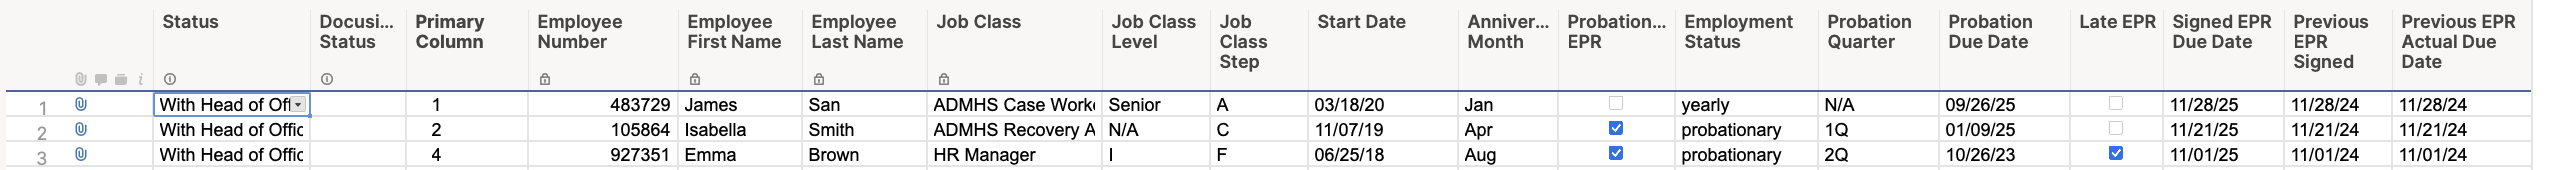
\includegraphics[width=\linewidth]{EPR Data 1.png}
    \caption{EPR 1}
    \label{fig:EPR1}
\end{figure}

\begin{figure}[H]
    \centering
    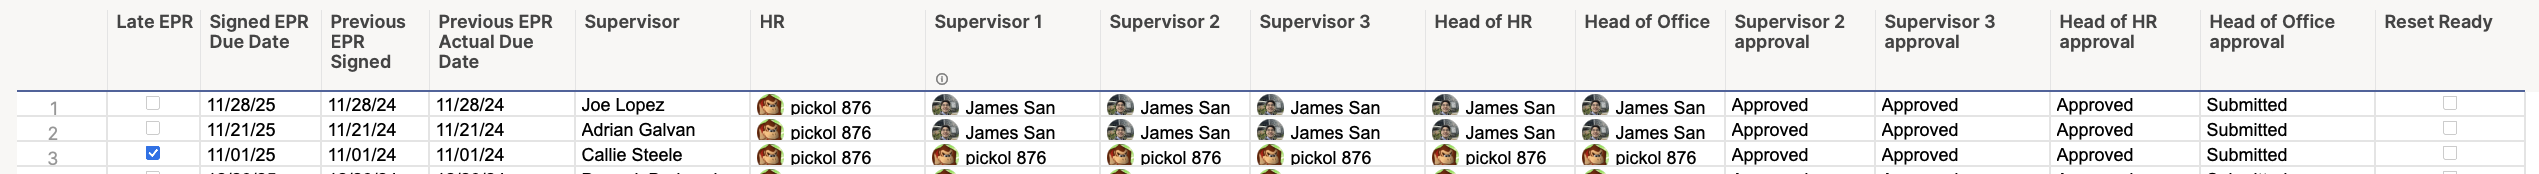
\includegraphics[width=\linewidth]{EPR Data 2.png}
    \caption{EPR 2}
    \label{fig:EPR2}
\end{figure}

\subsubsection{EPR Tracker - Employees History Records}

\textbf{Purpose:} Tracks the processing status of EPR records, including document handling (e.g., DocuSign), review progress, and approval workflow.

\textbf{Key Fields (Grouped):}
\begin{itemize}
    \item \textbf{Processing Info:} Date Saved, Status, DocuSign Status, Primary Column
    \item \textbf{Employee Info:} Employee Name, Job Class, Level, Step
    \item \textbf{EPR Details:} Anniversary Month, Probation Info, Due Dates, Late EPR
    \item \textbf{Assignments:} Supervisor(s), HR, Head of HR, Head of Office
    \item \textbf{Approvals:} Supervisor, HR, and Head of Office approval statuses
    \item \textbf{Tracking:} Previous EPR dates, Employment Status, Reset Ready flag
\end{itemize}

\textbf{Constraints:}
\begin{itemize}
    \item Only authorized roles can update status and approval fields.
\end{itemize}

\begin{figure}[H]
    \centering
    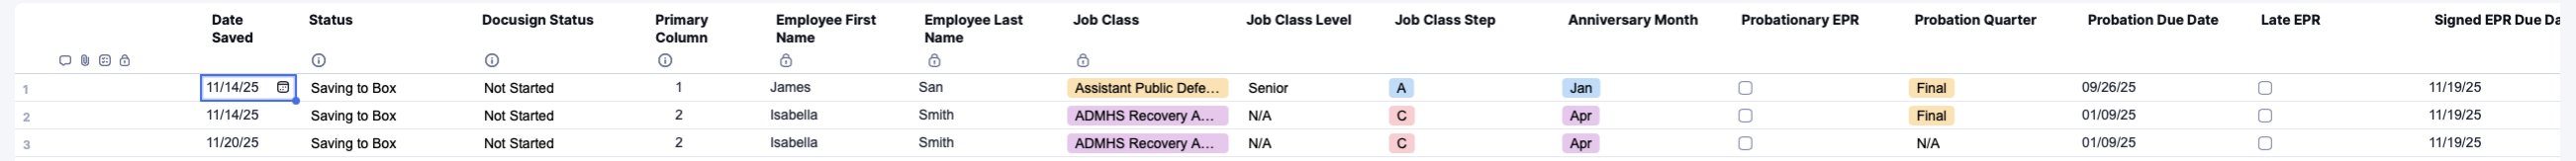
\includegraphics[width=\linewidth]{EPR Data History 1.png}
    \caption{EPR History 1}
    \label{fig:EPR_History1}
\end{figure}

\begin{figure}[H]
    \centering
    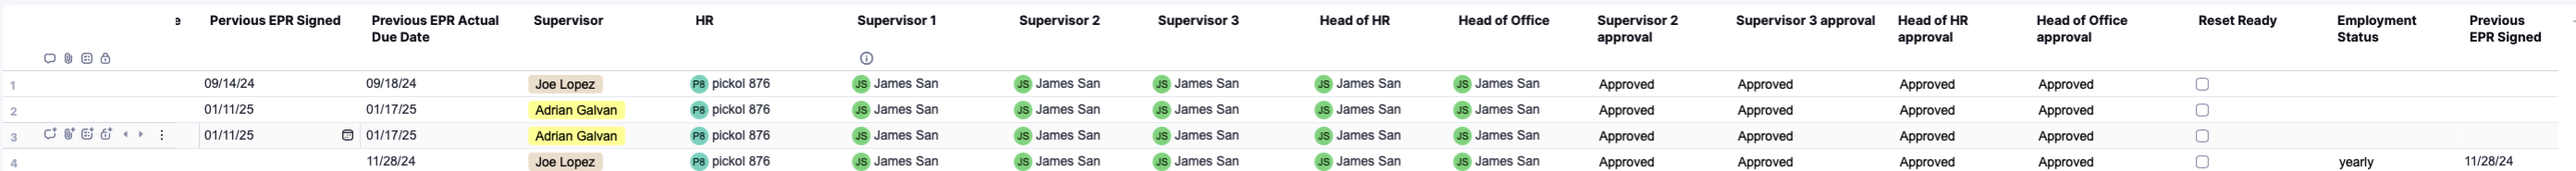
\includegraphics[width=\linewidth]{EPR Data History 2.png}
    \caption{EPR History 2}
    \label{fig:EPR_History2}
\end{figure}

\subsubsection{Personnel Matters - Personnel Matters Tracker}

\textbf{Purpose:} Tracks employee relations cases, including complaints, investigation details, status, and outcomes.

\textbf{Key Fields (Grouped):}
\begin{itemize}
    \item \textbf{Case Info:} Matter ID, Opened Date, Status, Days Open
    \item \textbf{Complaint Details:} Complaint Type, Issue, Policy, Description of Incident
    \item \textbf{People Involved:} Respondent, Supervisor, Intake Submitted Via
    \item \textbf{Case Management:} Next Steps, Due Dates, Memo Notes
    \item \textbf{Outcome \& Closure:} Closed Date, Outcome, Missing Close Info
    \item \textbf{Tracking:} Modified By, Last Modified Date, Fiscal Year, Update Required
\end{itemize}

\textbf{Constraints:}
\begin{itemize}
    \item Sensitive fields are restricted to authorized HR personnel.
\end{itemize}

\begin{figure}[H]
    \centering
    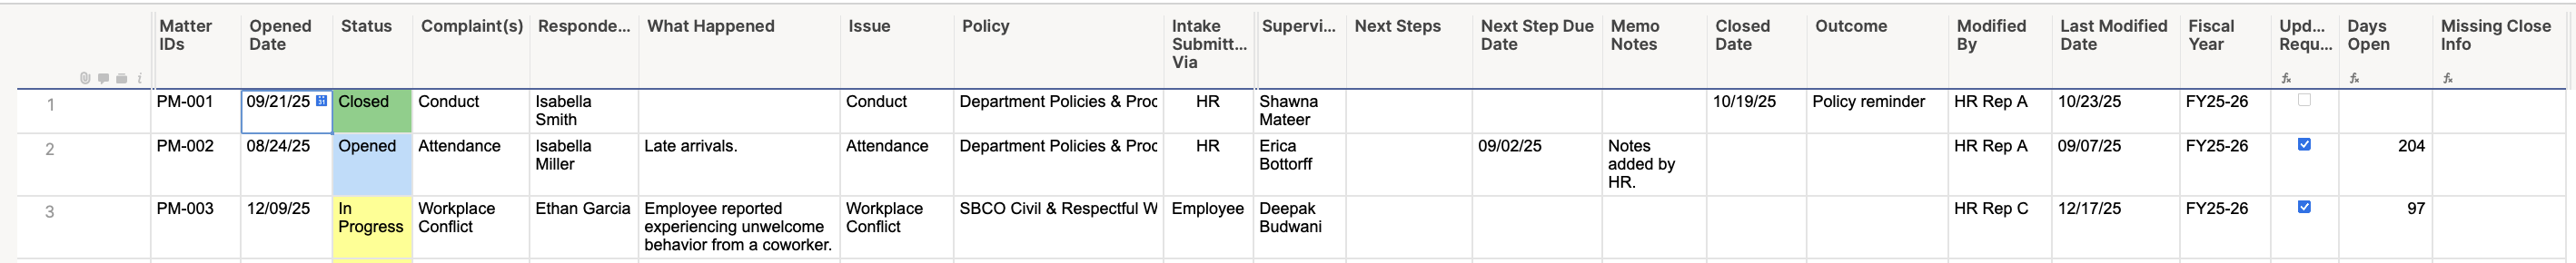
\includegraphics[width=\linewidth]{Personnel Matters Data.png}
    \caption{Personnel Matters Data}
    \label{fig:Personnel_Matters}
\end{figure}

\subsubsection{Separations - Employees Separations Tracker}

\textbf{Purpose:} Tracks employee separation records, including exit details, payroll timelines, and notification status.

\textbf{Key Fields (Grouped):}
\begin{itemize}
    \item \textbf{Submission Info:} Date Form Submitted, Separation ID, Email Status
    \item \textbf{Employee Info:} Employee ID, Name, Staff Email, Position ID, Job Class, Level
    \item \textbf{Separation Details:} Reason for Exit, Last Day Date
    \item \textbf{Payroll Tracking:} Pay Period, Payroll Start/End Dates, Final Pay Date
    \item \textbf{Benefits:} Insurance Last Date
\end{itemize}

\textbf{Constraints:}
\begin{itemize}
    \item Sensitive employee data is restricted to authorized HR personnel.
\end{itemize}

\begin{figure}[H]
    \centering
    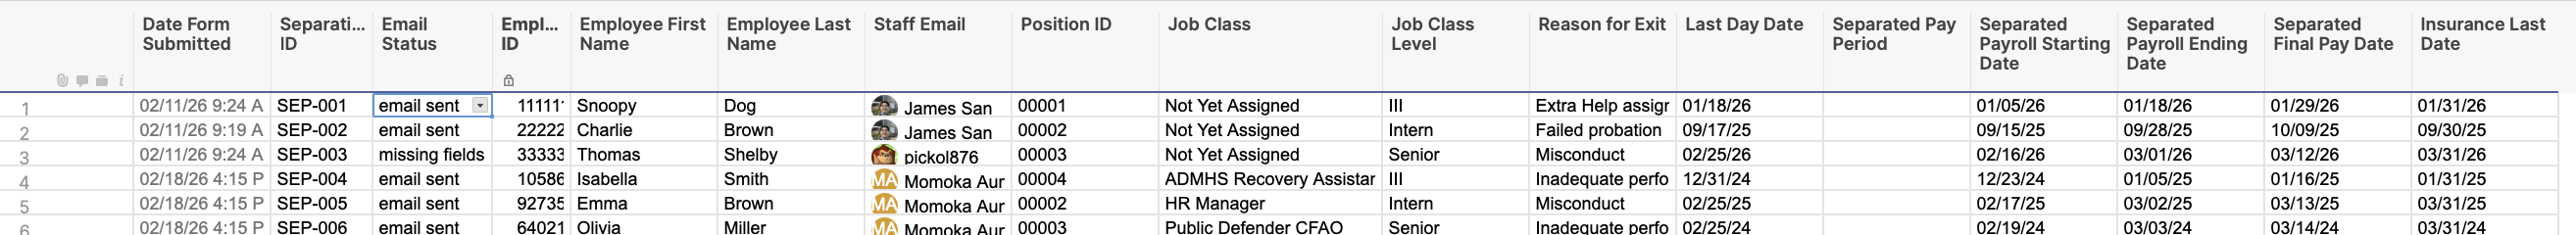
\includegraphics[width=\linewidth]{Separation Data.png}
    \caption{Separation Data}
    \label{fig:Separation}
\end{figure}

\subsubsection{Separations - Recognized Holidays}

\textbf{Purpose:} Maintains a list of organizational holidays, including dates and rules for recurring holidays.

\textbf{Key Fields (Grouped):}
\begin{itemize}
    \item \textbf{Holiday Info:} Holiday ID, Holiday Name
    \item \textbf{Dates:} Previous Holiday Date, Upcoming Holiday Date
    \item \textbf{Recurrence Rules:} Fixed Day Every Year, Fixed Day, Fixed Week of Month
\end{itemize}

\textbf{Constraints:}
\begin{itemize}
    \item Recurring holiday fields must be consistently defined for accurate date calculation.
\end{itemize}

\begin{figure}[H]
    \centering
    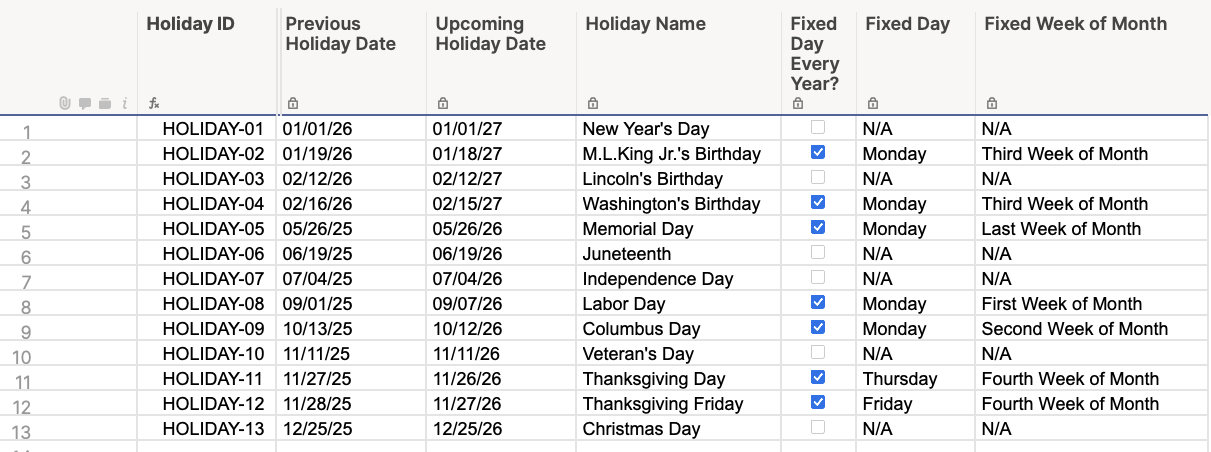
\includegraphics[width=\linewidth]{Separation Holiday Data.png}
    \caption{Separation Holiday Data}
    \label{fig:Separation_Holiday}
\end{figure}

\subsubsection{Vacancies and Recruitment - Vacancies and Recruitment}

\textbf{Purpose:} Tracks job vacancies, recruitment progress, and hiring activity.

\textbf{Key Fields (Grouped):}
\begin{itemize}
    \item \textbf{Vacancy Info:} Vacancy ID, Department, Position ID, Job Class Title
    \item \textbf{Status Tracking:} Status (e.g., Posted, Screening, Interviewing), Label
    \item \textbf{Timeline:} Vacancy Start Date, Date Filled, Vacancy Days Open
    \item \textbf{Recruitment Activity:} Recruitment Type, Interviews Conducted
    \item \textbf{System:} Row Created Timestamp
\end{itemize}

\textbf{Constraints:}
\begin{itemize}
    \item Limited by SharePoint list structure.
    \item Recruitment status fields are updated by authorized HR personnel only.
\end{itemize}

\begin{figure}[H]
    \centering
    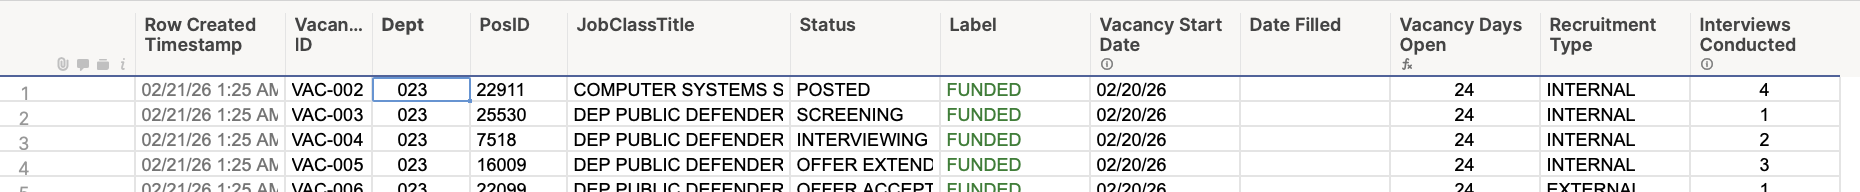
\includegraphics[width=\linewidth]{Vacancies and Recruitments Data.png}
    \caption{Vacancies and Recruitments Data}
    \label{fig:Vacancies_Recruitments}
\end{figure}

\noindent
This single-sheet data structure provides modularity, real-time synchronization, and high traceability while maintaining compliance with SBC PDO HR data governance policies.


% =====================================
% Section 10 – User Interface
% =====================================
\section{User Interface}

\subsection{Interface Overview}

The system does not implement a custom front-end application.  
User interaction occurs through three existing SaaS platforms:

\subsubsection{EPR}

\textbf{Smartsheet Interface and Notifications}

\begin{figure}[H]
    \centering
    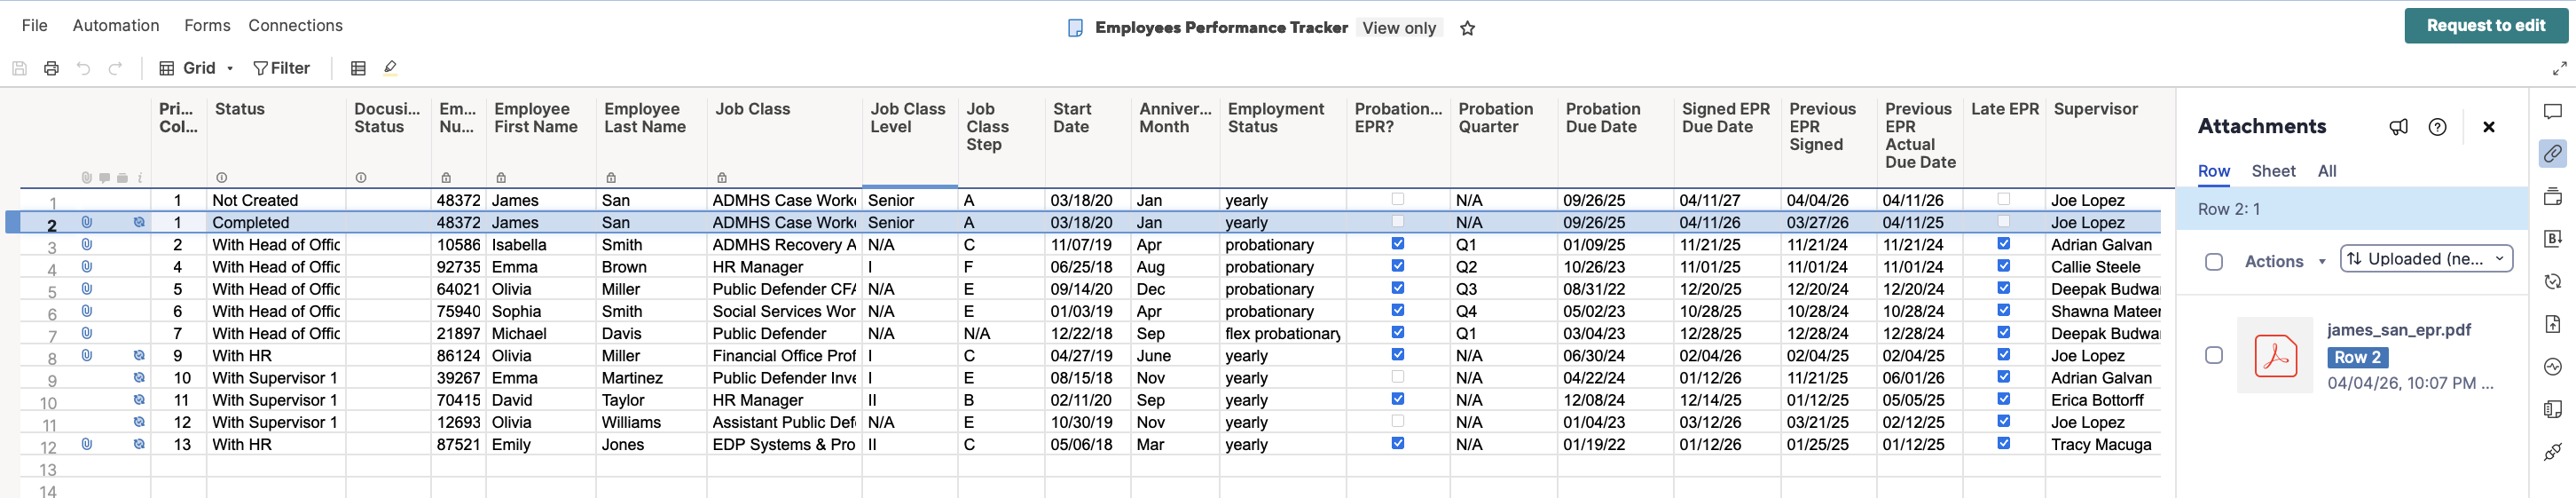
\includegraphics[width=0.8\linewidth]{EPR Smartsheet UI.png}
    \caption{EPR Smartsheet page}
    \label{fig:epr-smartsheet}
\end{figure}

\begin{figure}[H]
    \centering
    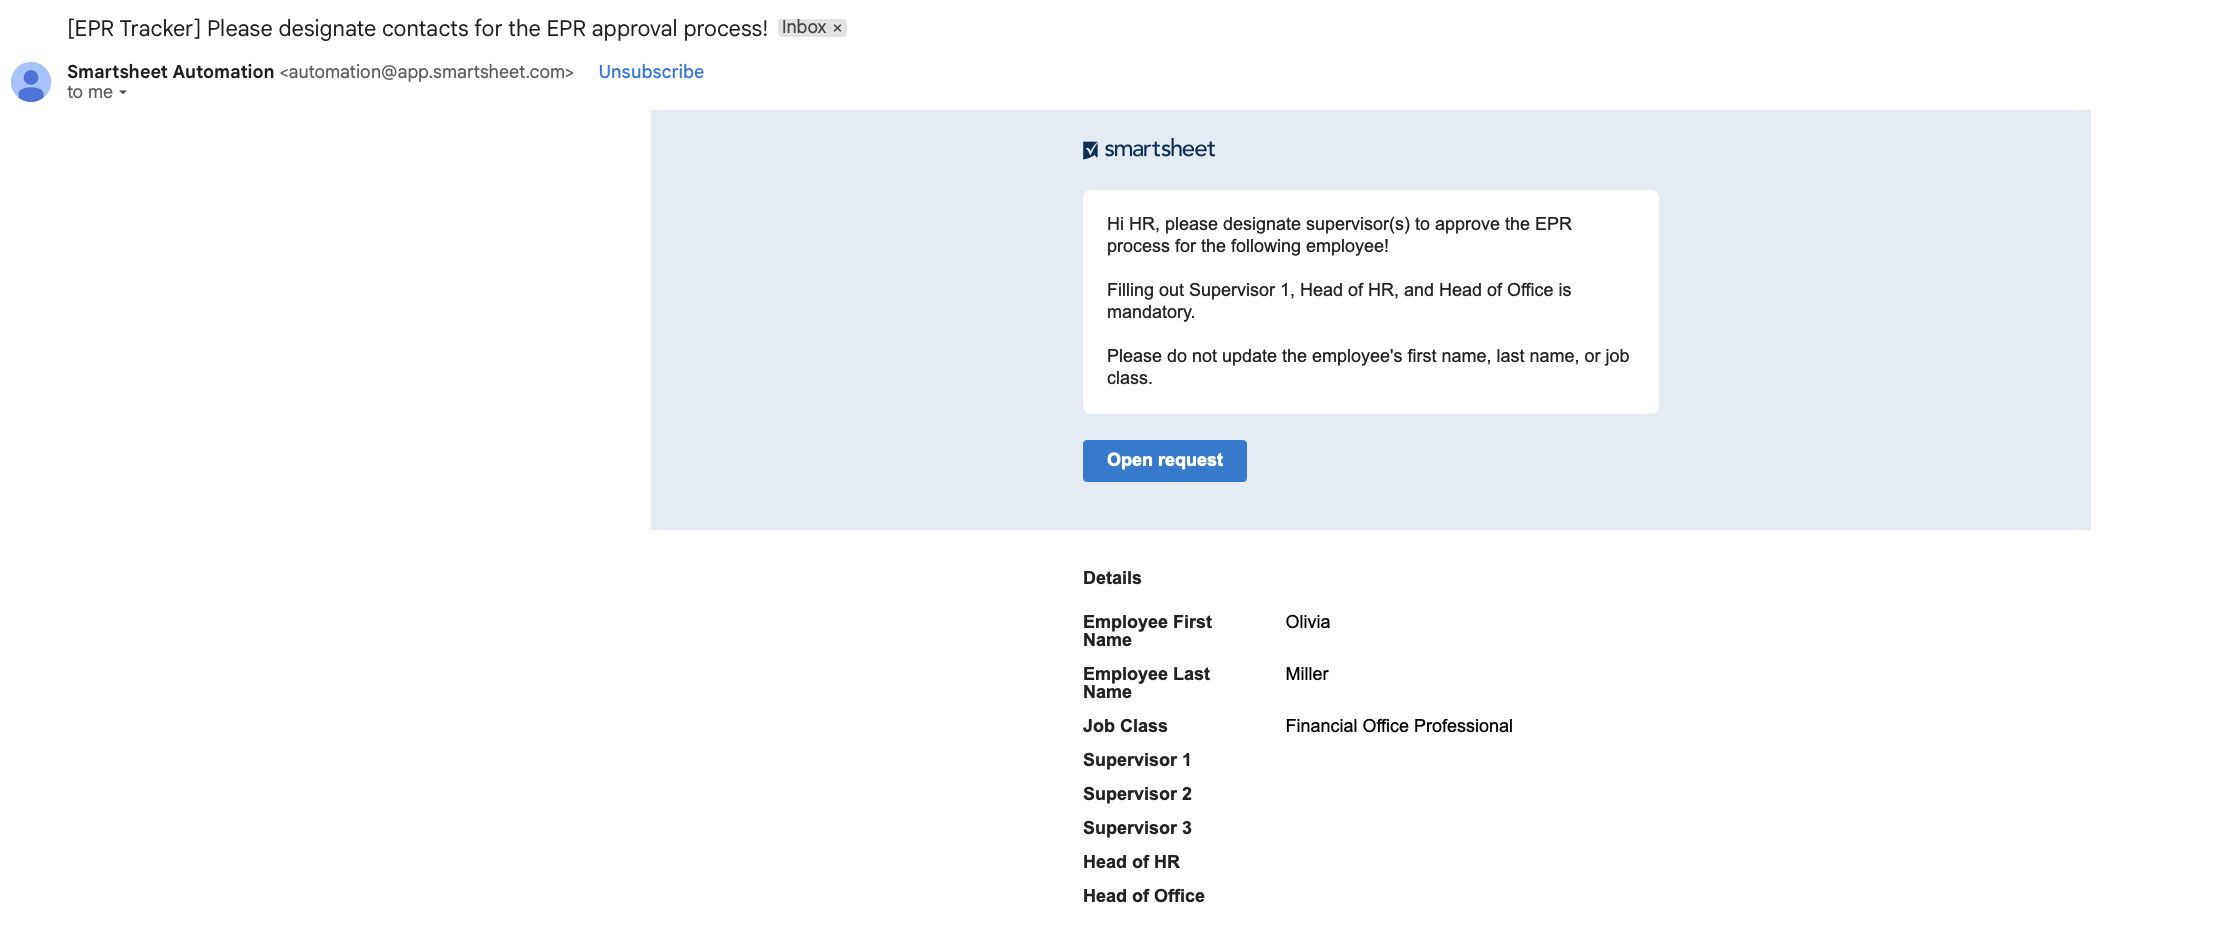
\includegraphics[width=0.8\linewidth]{EPR HR email.png}
    \caption{Automated Smartsheet emails prompting data from HR}
    \label{fig:epr-hr-email}
\end{figure}

\begin{figure}[H]
    \centering
    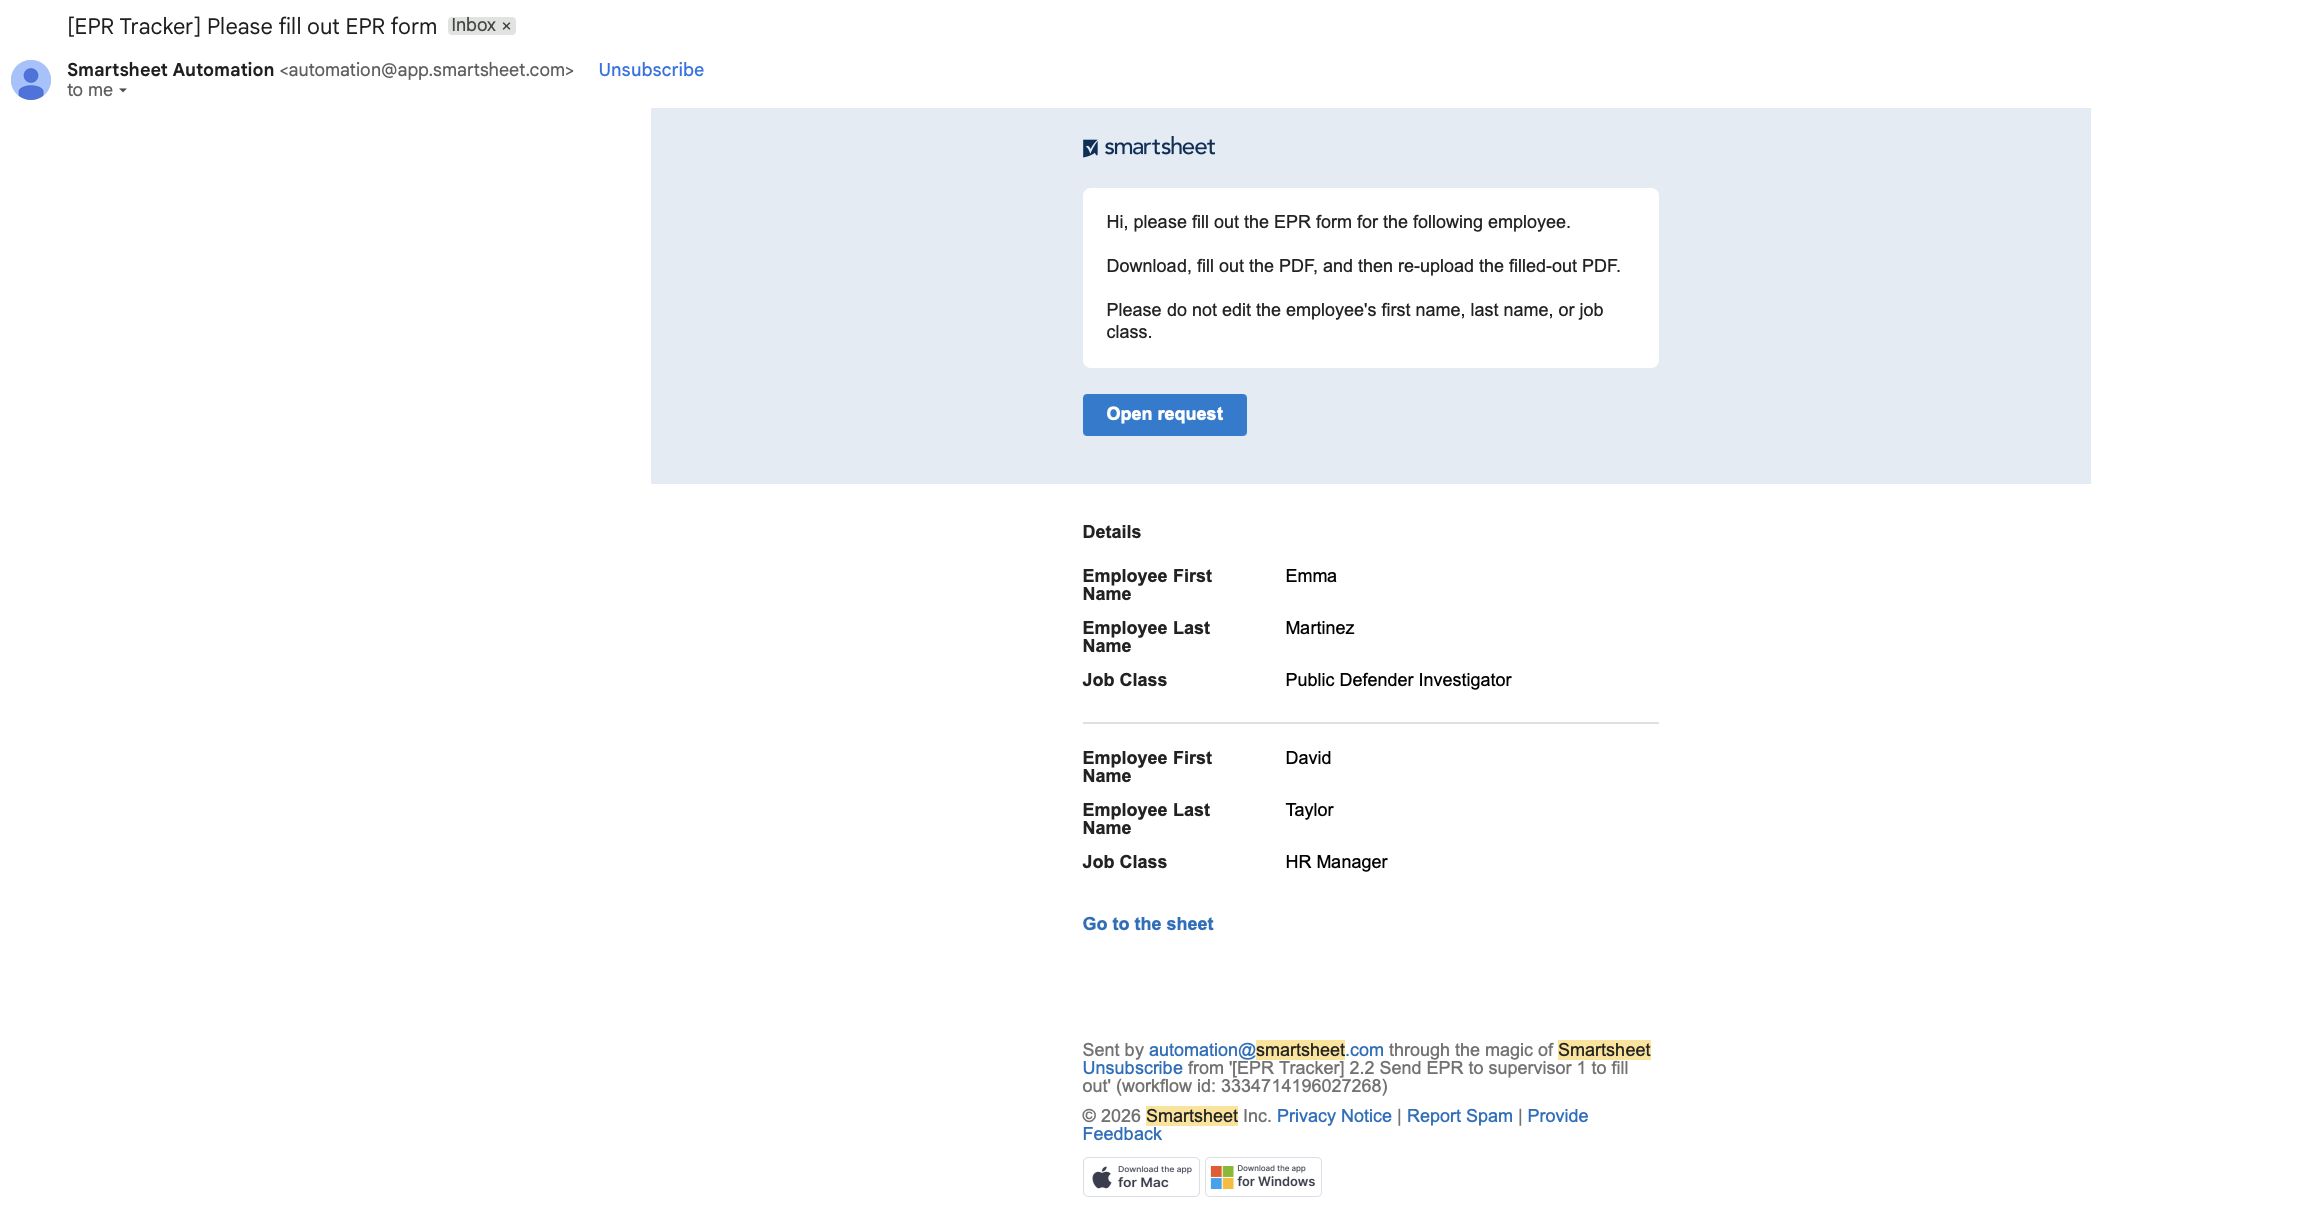
\includegraphics[width=0.8\linewidth]{EPR Supervisor email.png}
    \caption{Smartsheet-generated email prompting user actions}
    \label{fig:epr-prompting-email}
\end{figure}

\textbf{Power BI Dashboard}

The EPR Analytics Dashboard in Power BI provides near real-time insights into staffing and Employee Performance Review (EPR) progress. Data is refreshed nightly from Smartsheet.

\subparagraph{Page 1 -- HR Overview}

\textbf{Purpose:}  
Provide a high-level view of workforce structure, job classifications, and reporting relationships.

\textbf{Key Features:}
\begin{itemize}
    \item \textbf{Summary Cards (Employees, Supervisors, Interns, Employees on Probation)}  
    Displays key workforce metrics that dynamically update based on filters and slicers.

    \item \textbf{Find Employee (Search Slicer)}  
    Allows users to search and filter the dashboard by one or more employees.

    \item \textbf{Employee Directory}  
    A table showing Full Name, Job Class, Job Class Level, and Supervisor. Selecting a row filters other visuals.

    \item \textbf{Employees by Job Class Level}  
    Bar chart showing distribution across levels (Intern, I, II, III, Senior).

    \item \textbf{Employees by Job Class}  
    Horizontal bar chart displaying employee counts by job category.

    \item \textbf{Employees by Job Class and Level (Stacked Bar Chart)}  
    Combined visualization showing employee count by job class segmented by level.
\end{itemize}

\textbf{Use:}  
Supports workforce analysis, staffing distribution insights, and organizational planning.

\subparagraph{Page 2 -- EPR Performance Review}

\textbf{Purpose:}  
Track the status and completion of Employee Performance Reviews.

\textbf{Key Features:}
\begin{itemize}
    \item \textbf{Date Range Filter}  
    Allows users to view EPRs within a selected time window.

    \item \textbf{KPI Cards}  
    Displays Open EPRs, Completed EPRs, Total EPRs, and Completion Rate.

    \item \textbf{Open vs. Completed by Month}  
    Line chart showing trends in review progress over time.

    \item \textbf{Open EPRs by Job Class}  
    Bar chart highlighting outstanding reviews by job category.
\end{itemize}

\textbf{Key Metrics:}
\begin{itemize}
    \item Completion Rate (\%) = Completed EPRs / Total EPRs
    \item Open EPRs = Reviews currently in progress
    \item Overdue EPRs = Reviews past due and not completed
\end{itemize}

\textbf{Use:}  
Helps HR and supervisors monitor review progress, identify overdue evaluations, and track completion performance.

\subsubsection{Personnel Matters}

\textbf{Smartsheet / Intake Interfaces}

\begin{figure}[H]
    \centering
    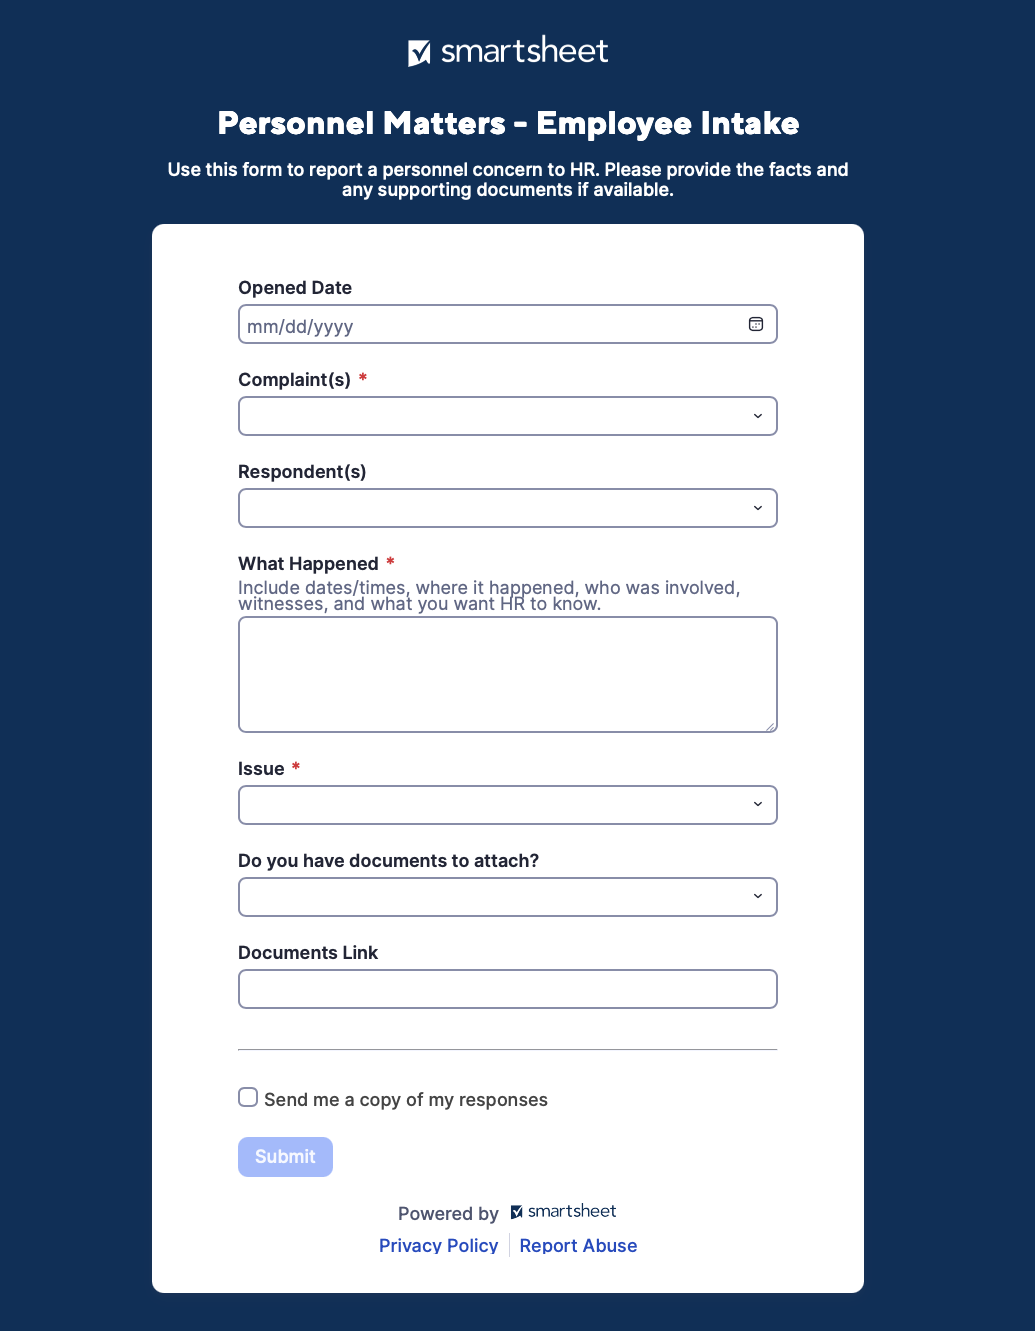
\includegraphics[width=0.4\linewidth]{Personnel Matters Employee Intake Form.png}
    \caption{Personnel Matters Employee Intake Form}
    \label{fig:personnel-intake-form}
\end{figure}

\begin{figure}[H]
    \centering
    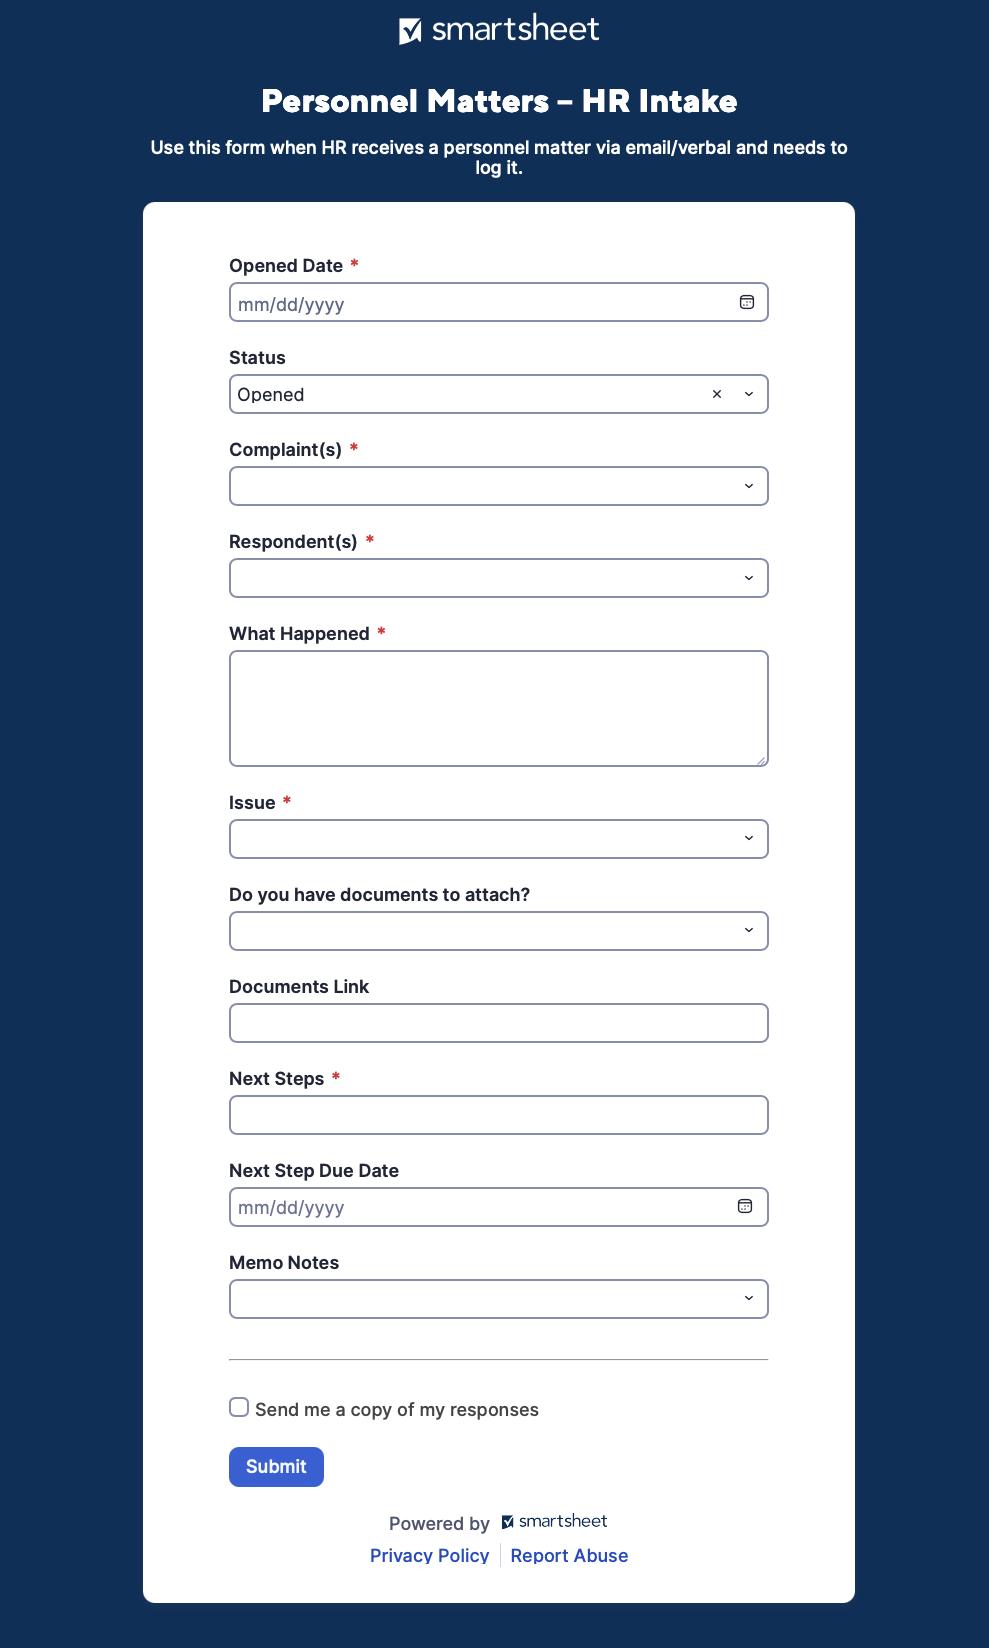
\includegraphics[width=0.4\linewidth]{Personnel Matters HR Intake Form.png}
    \caption{Personnel Matters HR Intake Form}
    \label{fig:personnel-matters-hr-intake-form}
\end{figure}

\textbf{Smartsheet / Data Tracker Interface}

\begin{figure}
    \centering
    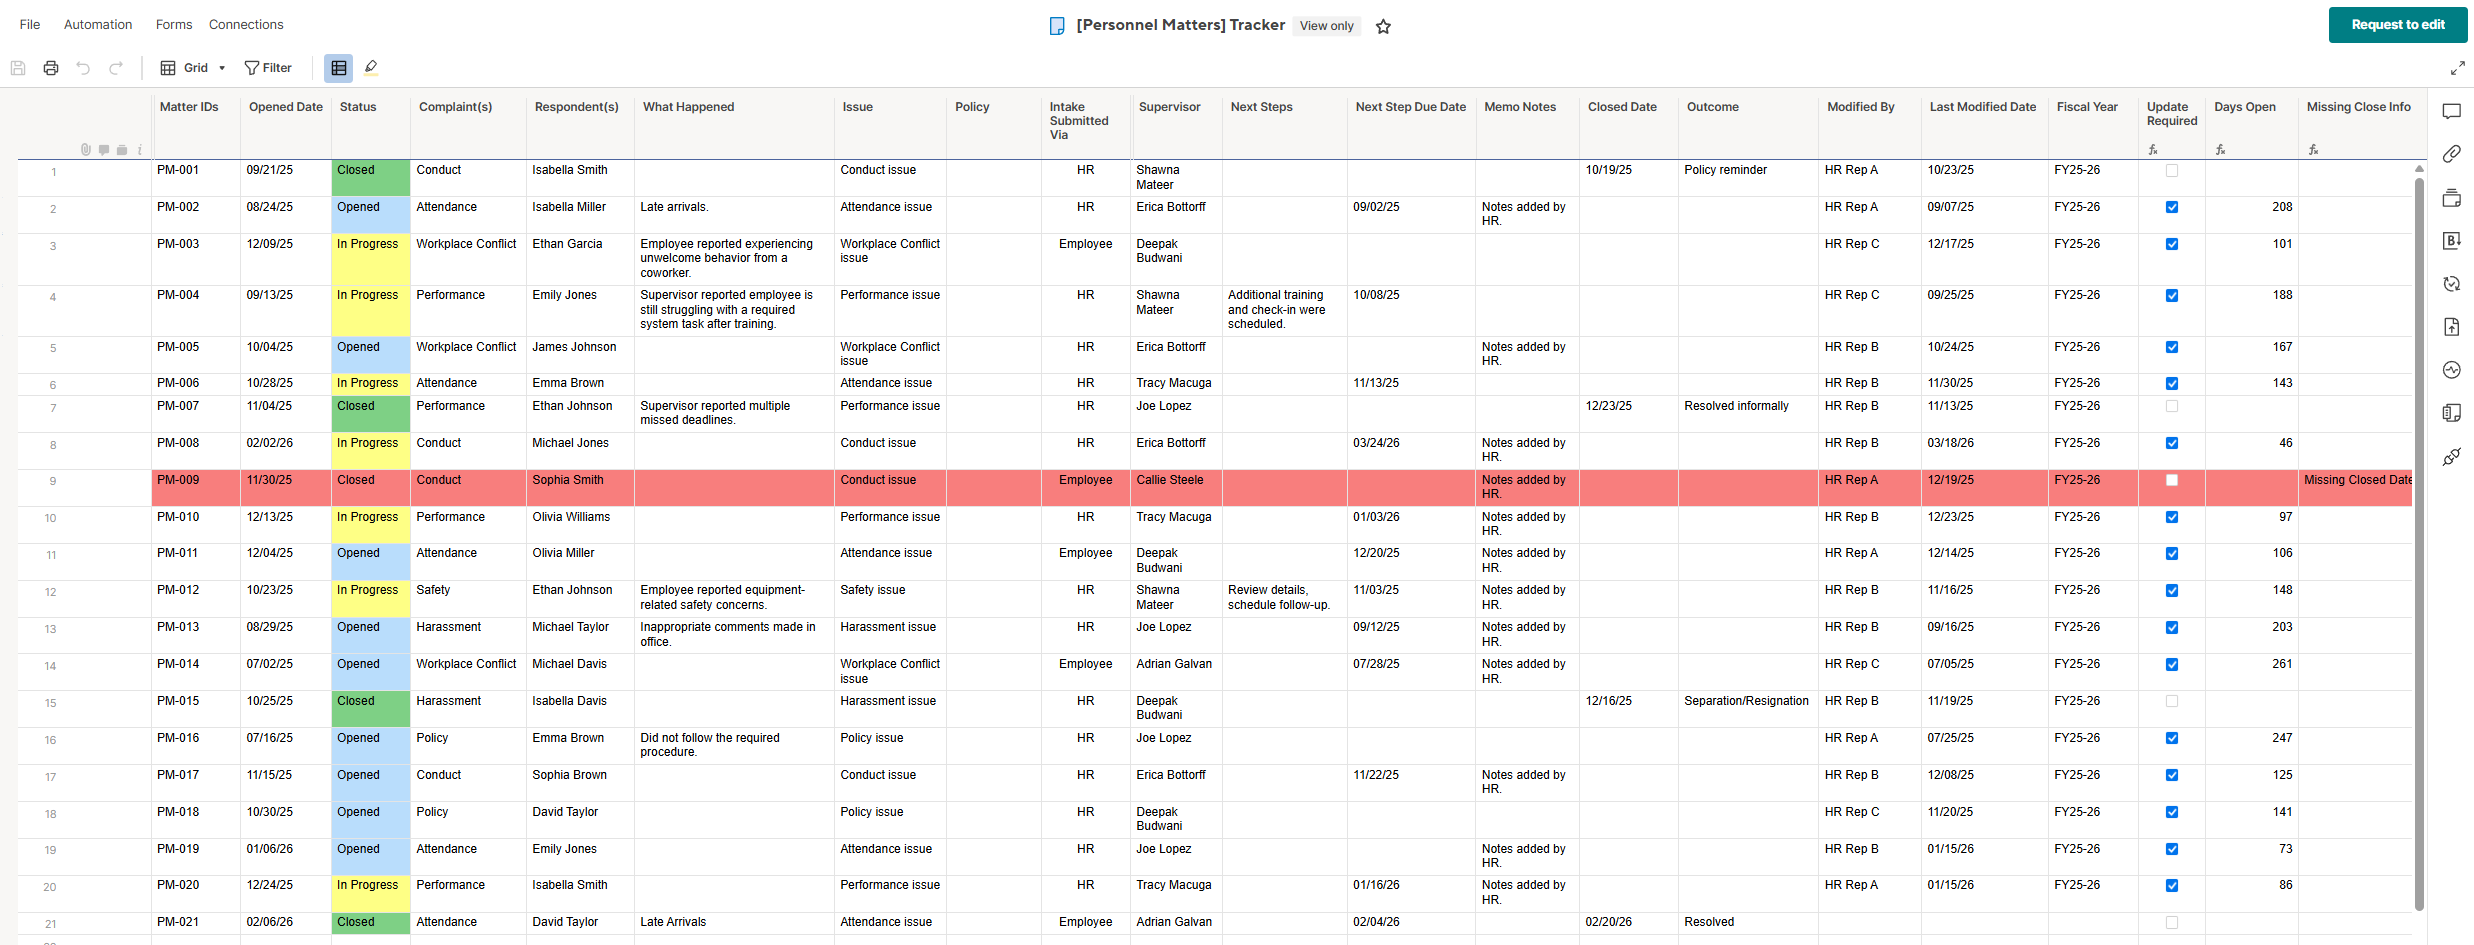
\includegraphics[width=1\linewidth]{Smartsheet Personnel Matters.png}
    \caption{Personnel Matters Smartsheet Data Overview}
    \label{fig:placeholder}
\end{figure}

The Personnel Matters Smartsheet tracker serves as the operational data source for this component. 
It stores case-level records submitted through intake forms and maintained by HR, including fields such as 
Matter ID, Opened Date, Status, Complaint Type, Respondent, Issue, Supervisor, Next Steps, Closed Date, 
Outcome, Days Open, and update-required indicators. This tracker supports case monitoring, follow-up actions, 
and downstream reporting in the Power BI dashboard.

\textbf{Power BI Dashboard}

\begin{figure}[H]
    \centering
    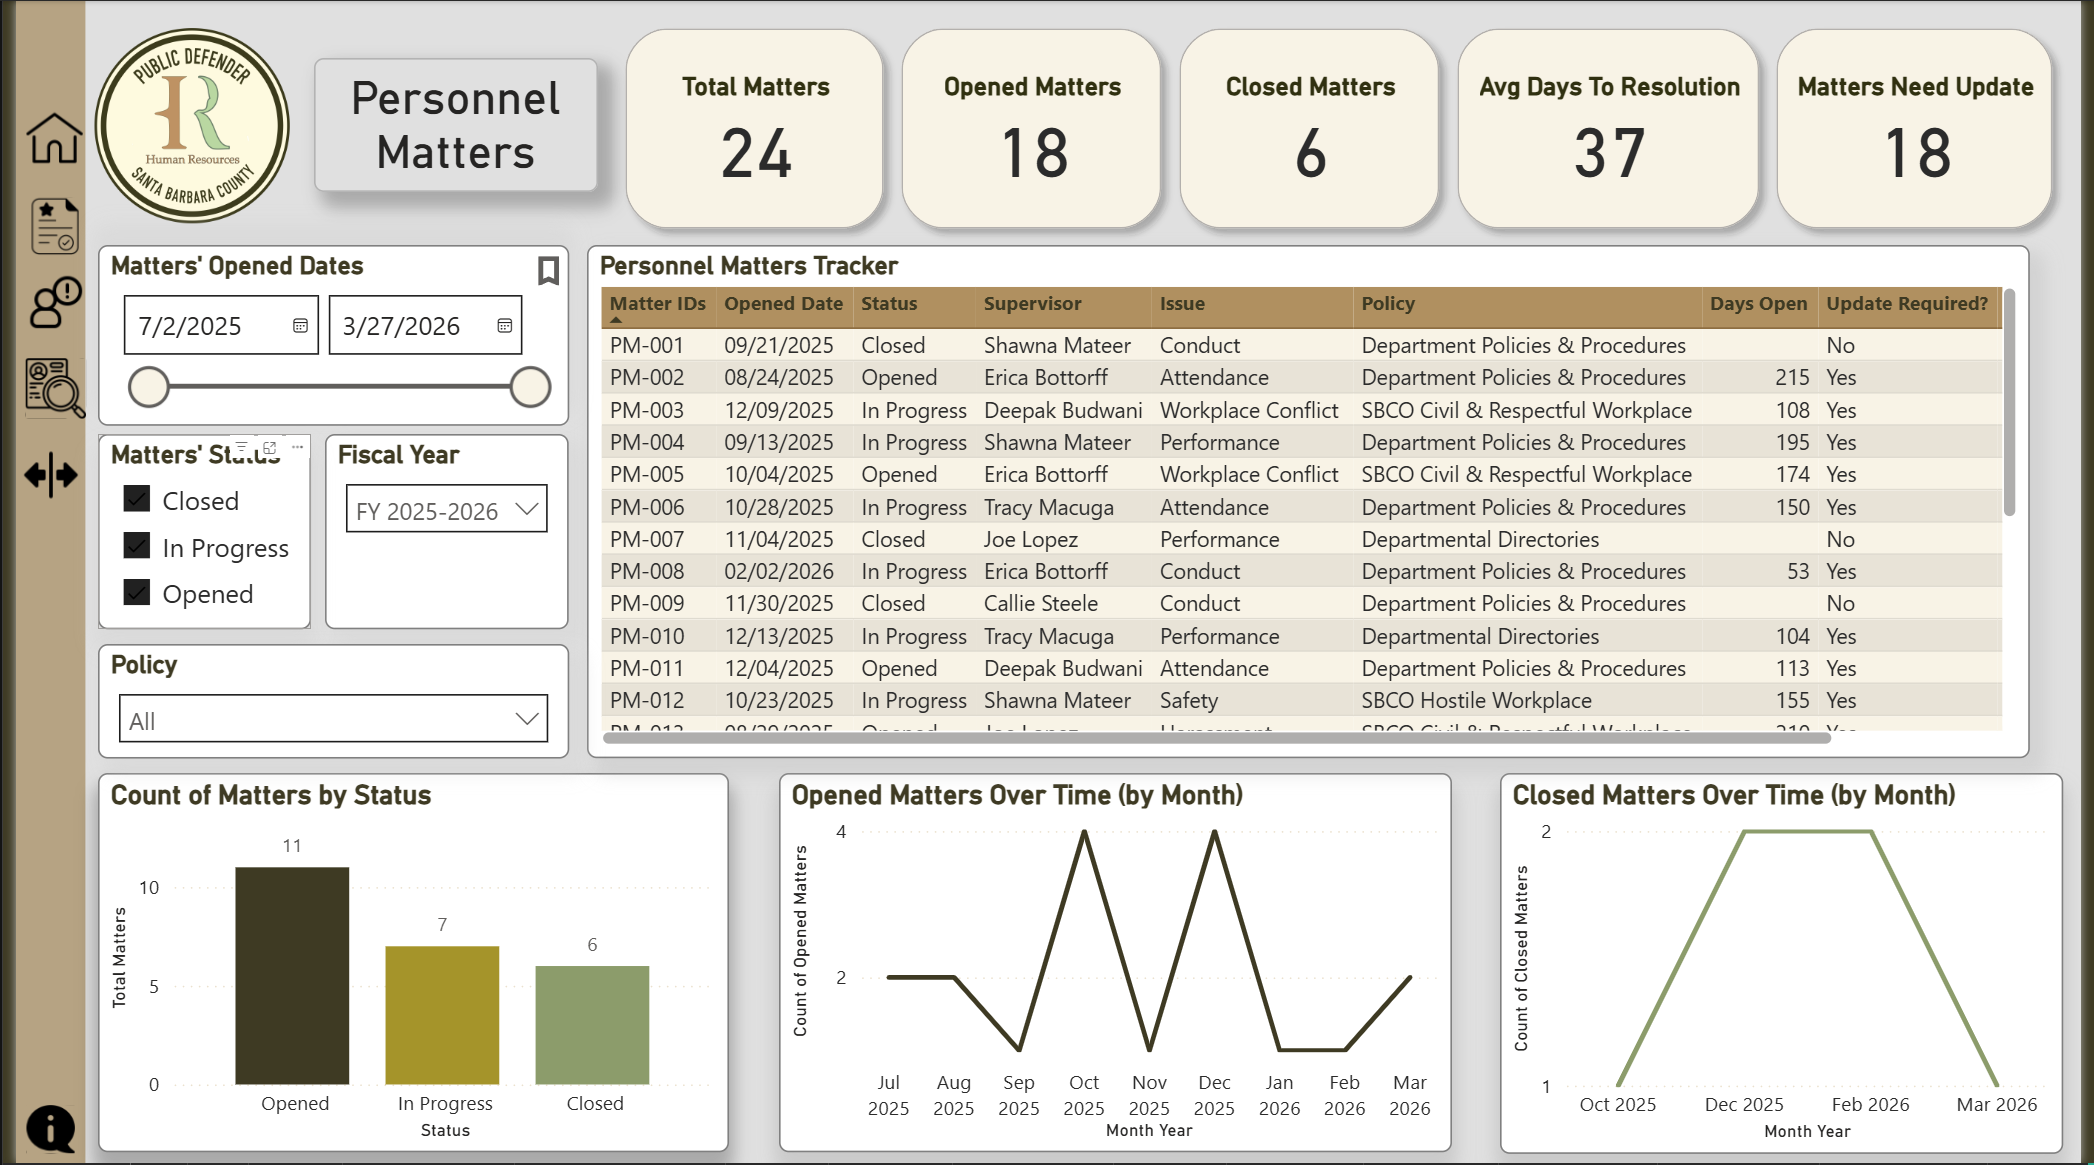
\includegraphics[width=0.95\linewidth]{PowerBI Dashboard Personnel Matters.png}
    \caption{Power BI Personnel Matters Dashboard}
    \label{fig:personnel-matters-dashboard}
\end{figure}


The Personnel Matters Dashboard in Power BI provides near real-time visibility into employee relations cases, including open matters, closed matters, case status, and resolution activity. Data is refreshed from the Personnel Matters Smartsheet tracker and supports filtering for targeted HR review and compliance monitoring.

\textbf{Overview Purpose:} Provide HR and leadership with a centralized view of personnel matters so they can monitor case volume, case status, overdue follow-up, and resolution trends.

\textbf{Key Features:}
\begin{itemize}
    \item \textbf{KPI Cards} display summary values such as Total Matters, Open Matters, Closed Matters, and Average Days to Resolution.
    \item \textbf{Status Breakdown} visual shows the distribution of cases by current status to help users quickly identify unresolved or in-progress matters.
    \item \textbf{Matters Opened Over Time} chart displays monthly or yearly intake trends for personnel matters.
    \item \textbf{Matters Closed Over Time} chart shows case resolution activity across time.
    \item \textbf{Detailed Tracker Table} displays case-level information such as Matter ID, Opened Date, Status, Complaint Type, Supervisor, and Closed Date.
    \item \textbf{Filter Controls} allow users to refine the dashboard by date range, fiscal year, status, complaint category, supervisor, or intake method.
\end{itemize}

\textbf{Use:} Helps HR monitor case progress, identify overdue or unresolved matters, support compliance reporting, and improve visibility into employee relations.

\subsubsection{Vacancies and Recruitment}

\textbf{Smartsheet / Data Import Interface}

The Vacancies and Recruitment component uses structured vacancy and recruitment data to support reporting on open positions, hiring progress, and workforce planning.

\begin{figure}[H]
    \centering
    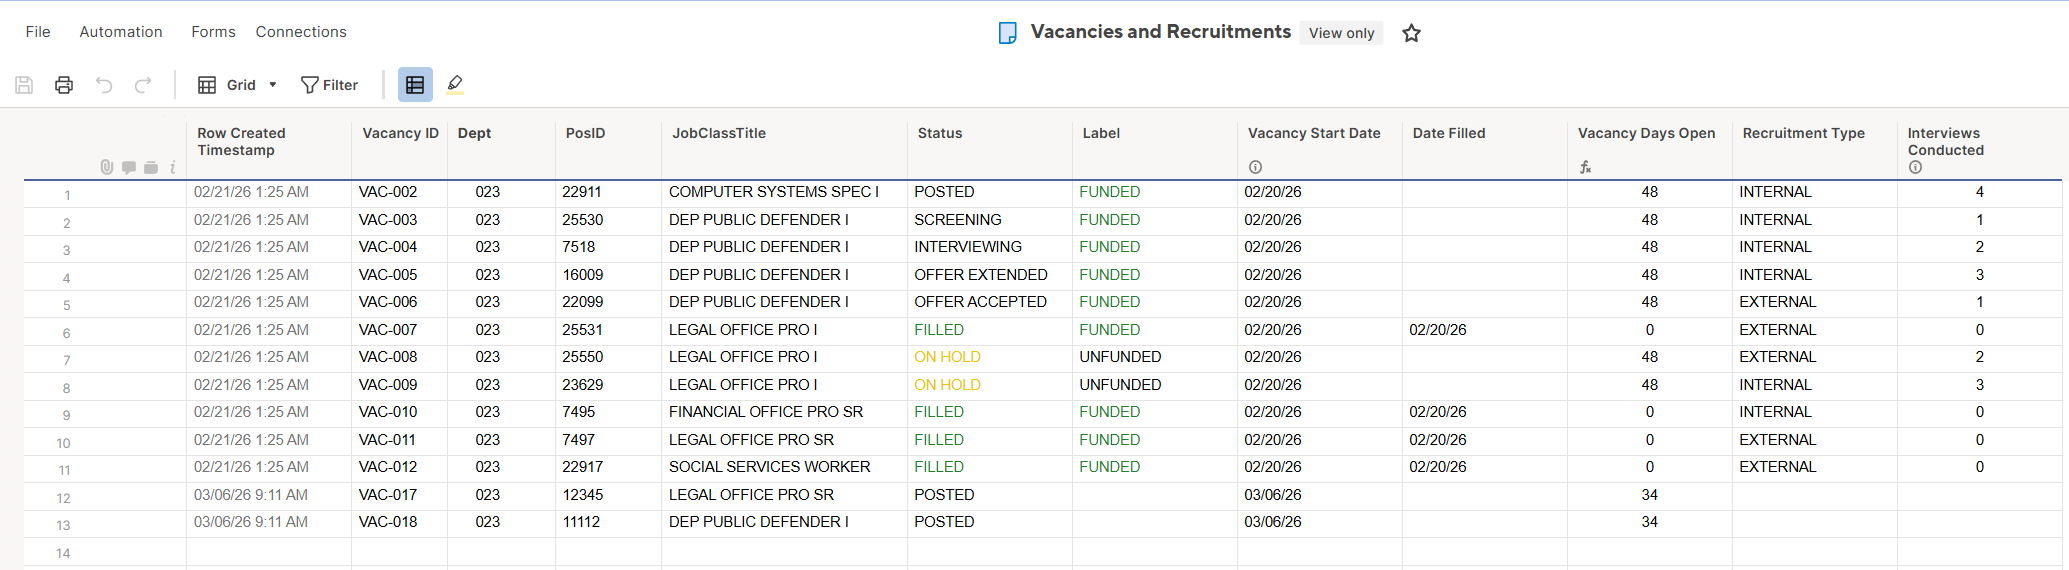
\includegraphics[width=0.95\linewidth]{Smartsheet Vacancies.png}
    \caption{Recruitment \& Vacancies Smartsheet Data}
    \label{fig:vacancies-smartsheet}
\end{figure}

\textbf{Power BI Dashboard}

\FloatBarrier

\begin{figure}[H]
    \centering
    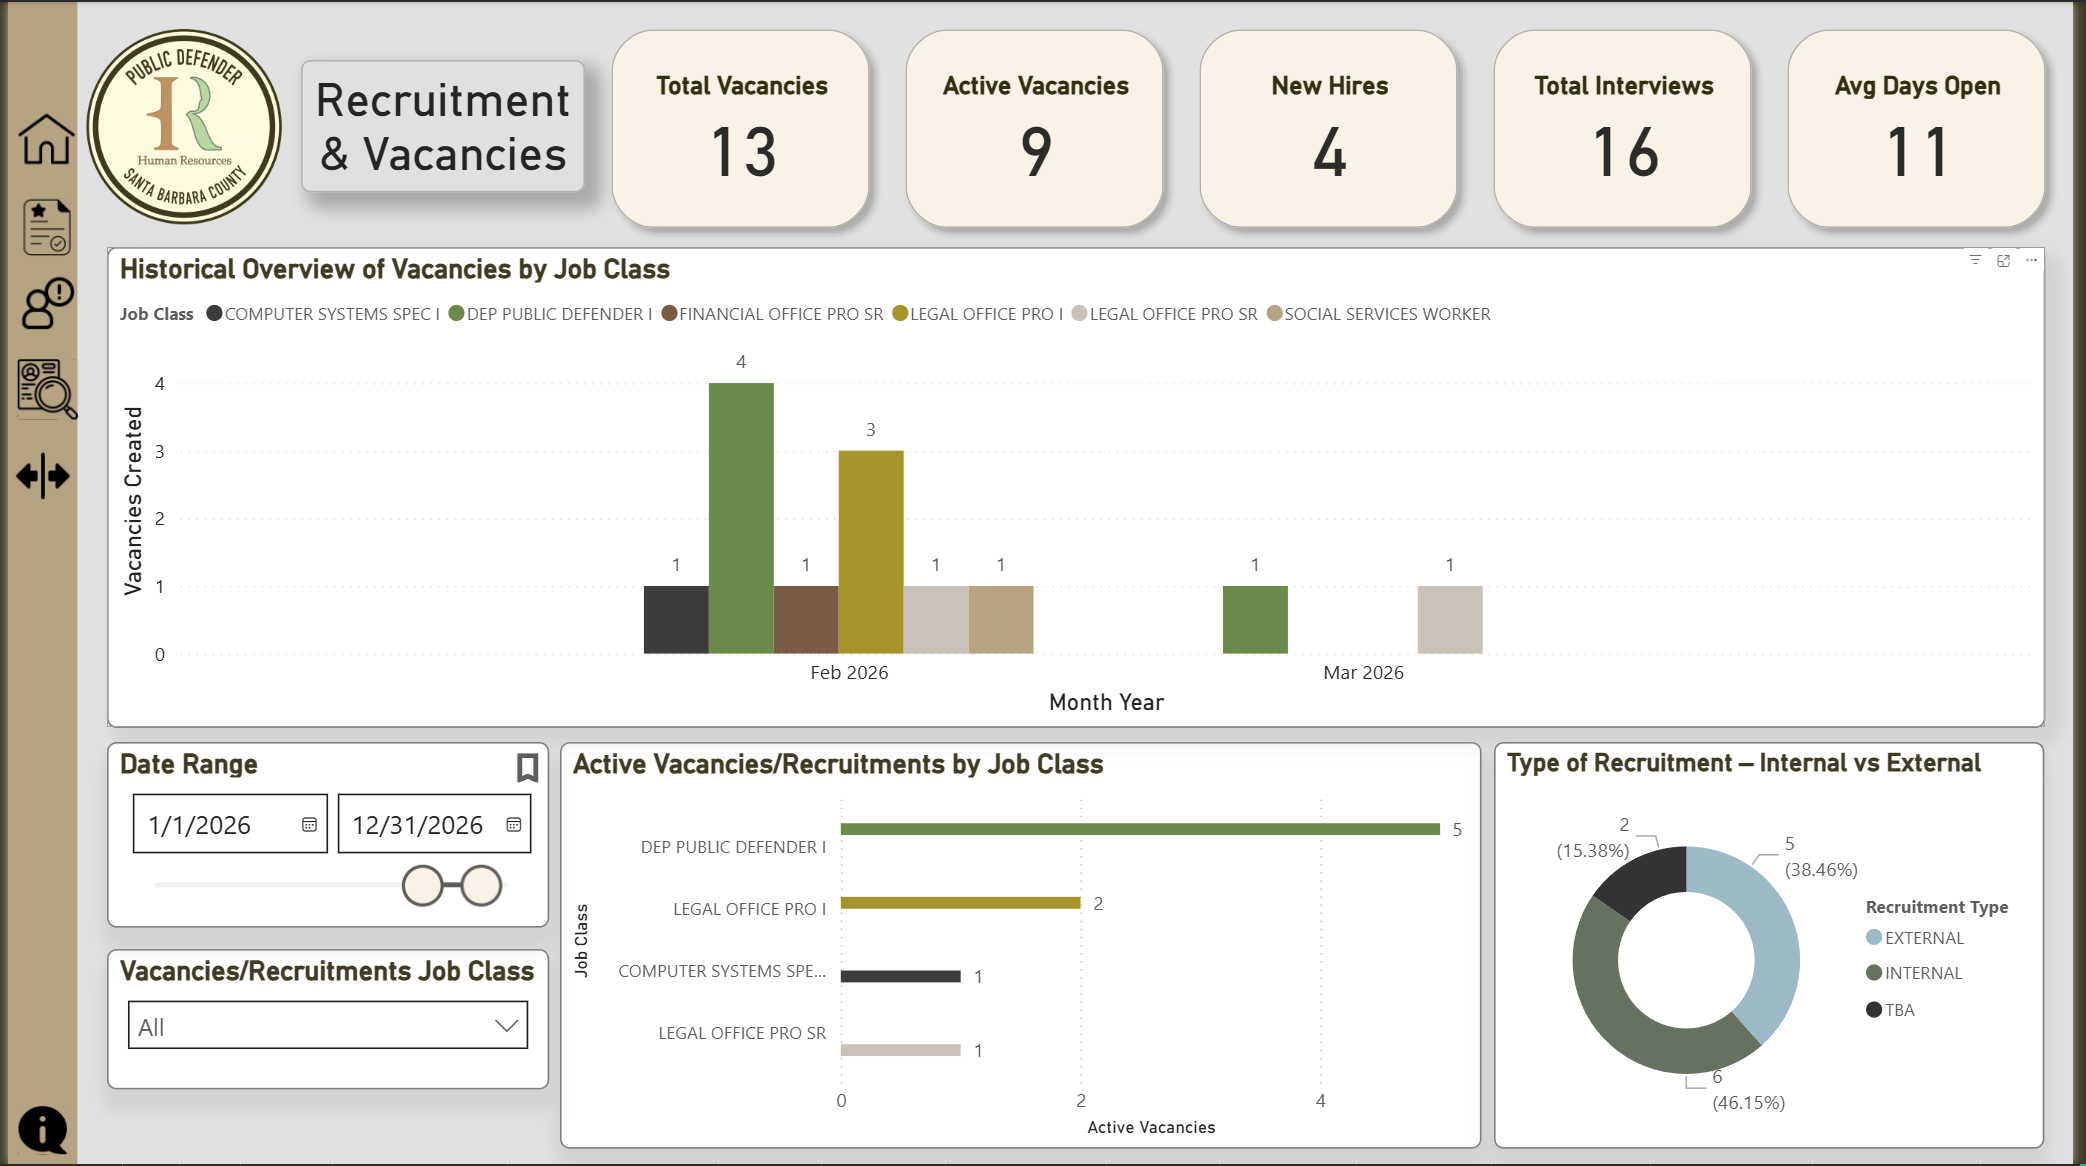
\includegraphics[width=0.95\linewidth]{PowerBI Dashboard Vacancies p1.png}
    \caption{Power BI Vacancies Dashboard Page 1}
    \label{fig:vacancies-dashboard-page1}
\end{figure}

\FloatBarrier

\paragraph{Page 1 --- Vacancies Overview}

\textbf{Purpose:} Provide a high-level view of current vacancy volume, active positions, and vacancy distribution across the organization.

\textbf{Key Features:}
\begin{itemize}
    \item \textbf{KPI Cards} display summary values such as Total Vacancies, Active Vacancies, Filled Vacancies, and average vacancy days open.
    \item \textbf{Active Vacancies by Job Class} visual highlights which job categories currently have the highest staffing need.
    \item \textbf{Vacancy Status Breakdown} visual displays positions by workflow stage, such as Posted, Screening, Interviewing, Offer Extended, or Filled.
    \item \textbf{Vacancy Trend Over Time} chart shows how vacancy volume changes across months or fiscal periods.
    \item \textbf{Additional categorical visuals} may show vacancy distribution by funding label, department, office location, or other available organizational fields.
    \item \textbf{Filter controls} allow users to refine the dashboard by date range, fiscal year, job class title, department, funding label, or vacancy status.
\end{itemize}

\textbf{Use:} Supports staffing analysis, hiring prioritization, and workforce planning by helping HR identify where vacancies are concentrated and how long positions remain open.

\paragraph{Page 2 --- Recruitment Overview}

\textbf{Purpose:} Track recruitment activity, hiring progress, and operational metrics related to filling positions.

\begin{figure}[H]
    \centering
    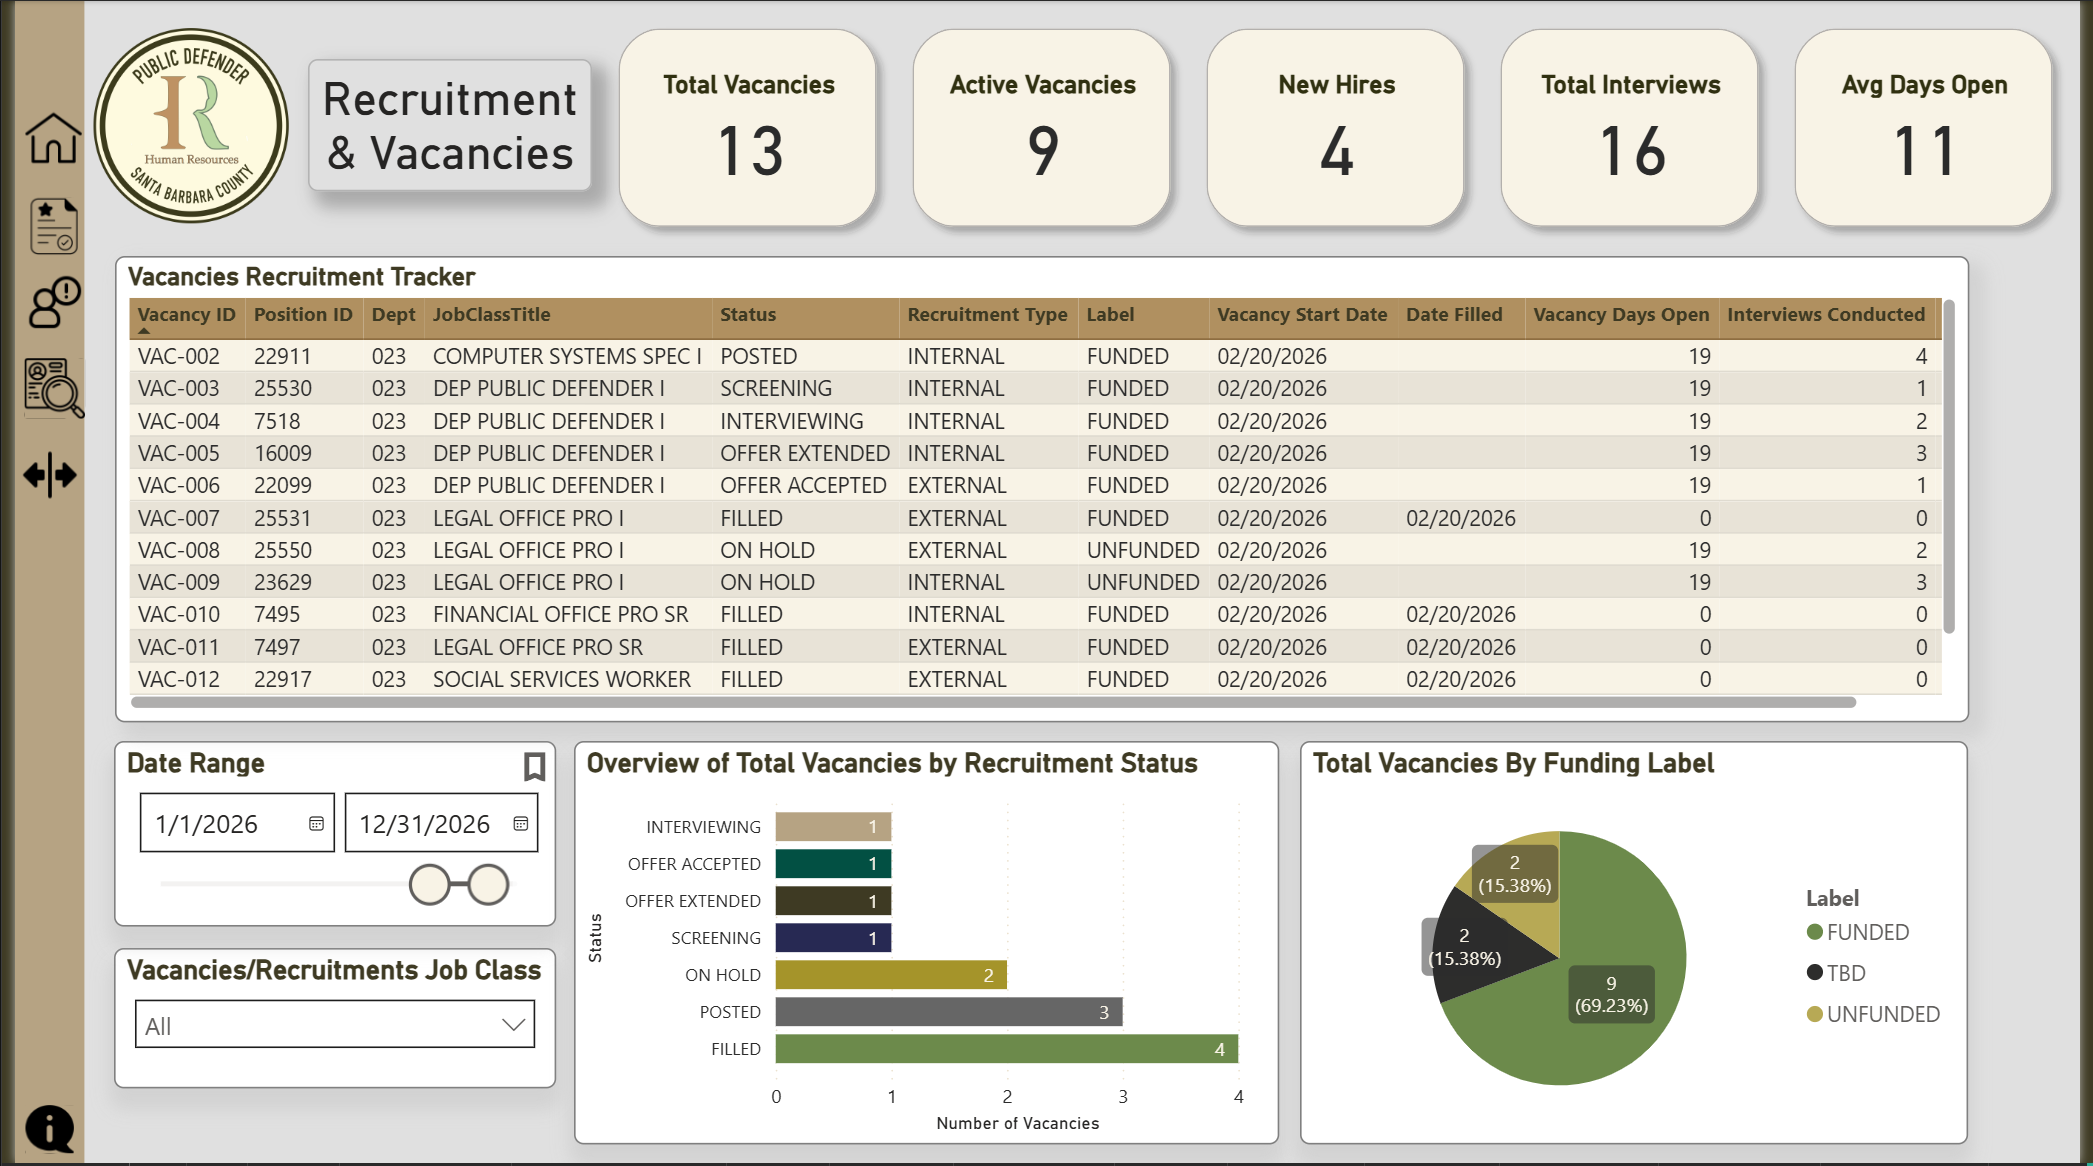
\includegraphics[width=0.95\linewidth]{PowerBI Dashboard Vacancies p2.png}
    \caption{Power BI Vacancies Dashboard Page 2}
    \label{fig:vacancies-dashboard-page2}
\end{figure}

\textbf{Key Features:}
\begin{itemize}
    \item \textbf{KPI Cards} display summary values such as Recruitment Records, Interviews Conducted, New Hires, or other hiring activity metrics available in the dataset.
    \item \textbf{Recruitment Type Breakdown} visual shows internal versus external recruitment activity when applicable.
    \item \textbf{Hiring Activity Over Time} chart displays recruitment and hiring trends across selected time periods.
    \item \textbf{Historical Overview by Job Class} visual helps HR compare recruitment volume and outcomes across classifications.
    \item \textbf{Detailed Recruitment Table} provides row-level visibility into vacancy ID, job class title, recruitment type, interviews conducted, date filled, and current status.
    \item \textbf{Shared Filters} allow users to analyze recruitment data by job class, recruitment type, status, fiscal year, and date range.
\end{itemize}

\textbf{Use:} Helps HR track recruitment pipeline progress, monitor hiring outcomes, evaluate time-to-fill patterns, and support operational hiring decisions.



\subsubsection{Separations}

\textbf{Smartsheet Form Interface}

\begin{figure}[H]
    \centering
    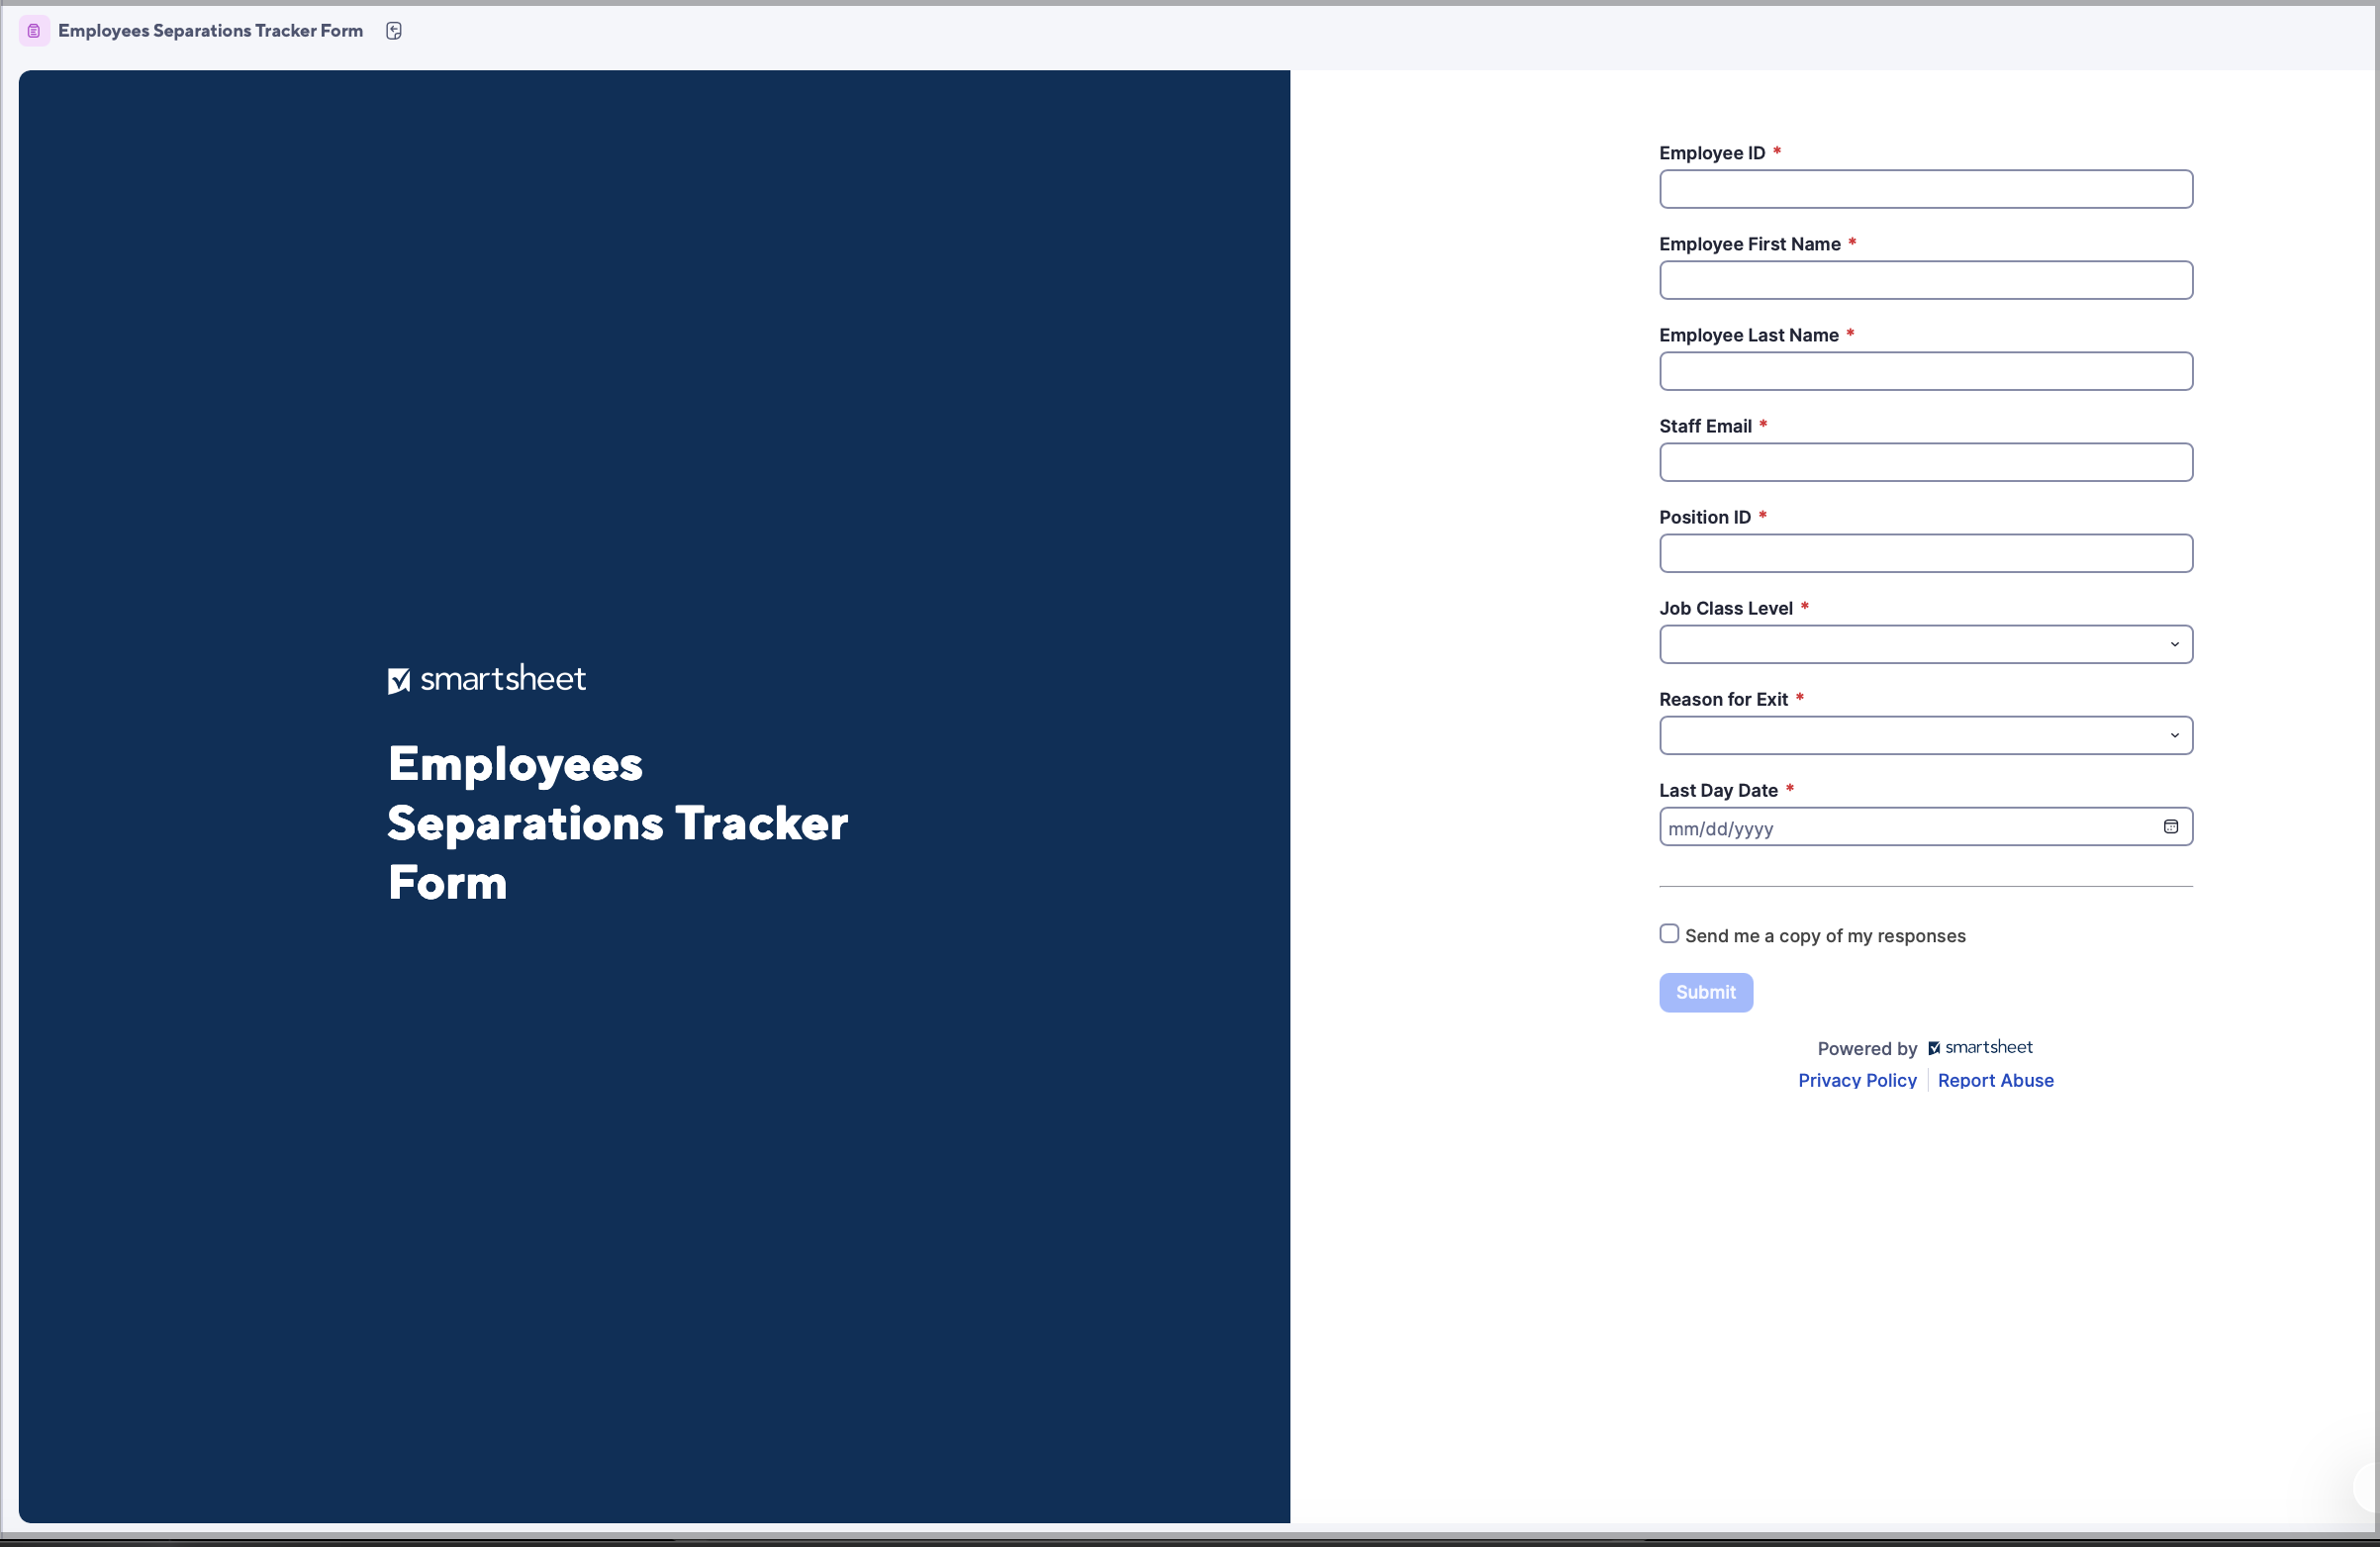
\includegraphics[width=0.8\linewidth]{Separation UI.png}
    \caption{Separation HR Intake Form}
    \label{fig:separation-hr-intake-form}
\end{figure}

\textbf{Separations Dashboard}

The Separations Dashboard in Power BI provides insights into employee separations, including total exits, reasons for leaving, and trends over time. The dashboard supports filtering by job class, fiscal year, and date range to enable flexible analysis.

\begin{figure}[H]
    \centering
    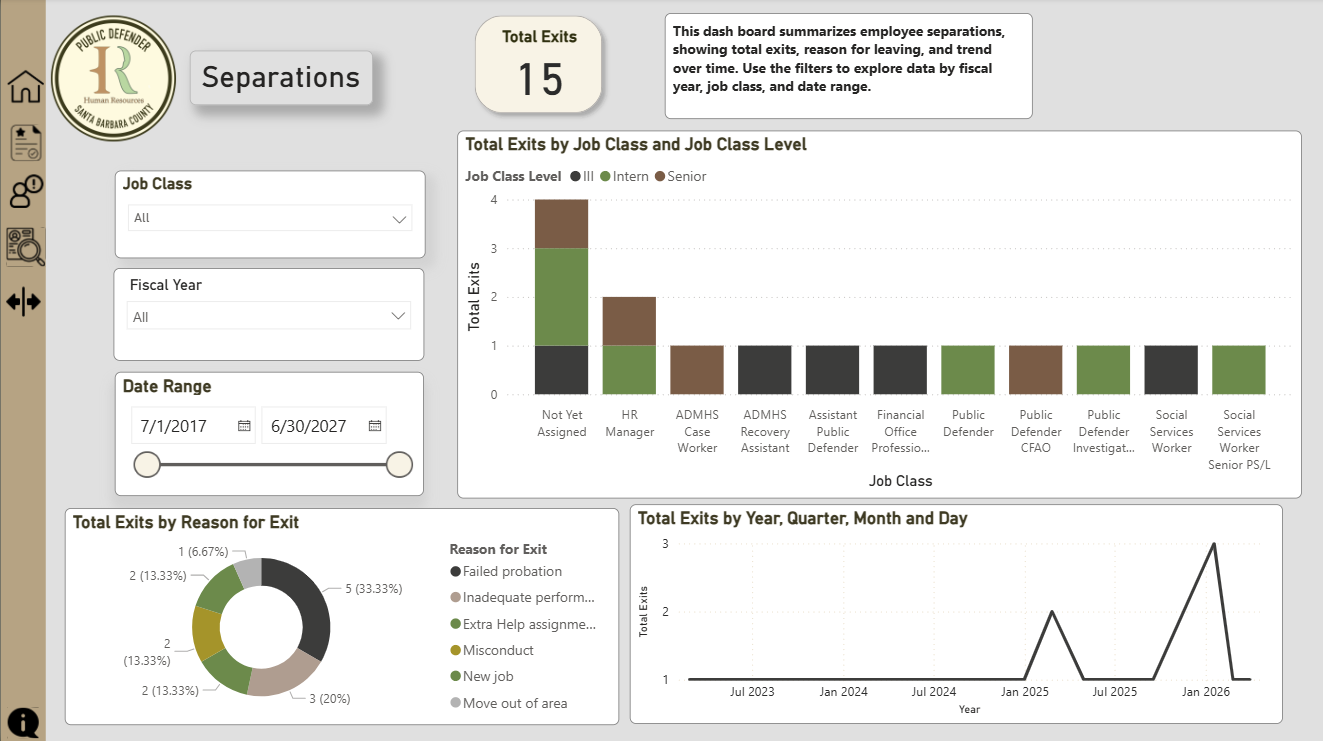
\includegraphics[width=0.8\linewidth]{Separation PBI.png}
    \caption{Separation PowerBI Dashboard}
    \label{fig:separation-pbi-dashboard}
\end{figure}

\subparagraph{Overview}

\textbf{Purpose:}  
Provide a comprehensive view of employee separations to support workforce planning, retention analysis, and organizational decision-making.

\textbf{Key Features:}
\begin{itemize}
    \item \textbf{Total Exits KPI}  
    Displays the total number of employee separations within the selected filters.

    \item \textbf{Filters (Job Class, Fiscal Year, Date Range)}  
    Allows users to refine the dataset dynamically for targeted analysis.

    \item \textbf{Total Exits by Job Class and Job Class Level}  
    Stacked bar chart showing separations across job classes, segmented by level (e.g., Intern, I, Senior).  
    \textit{Use:} Helps identify which roles and levels experience the highest turnover.

    \item \textbf{Total Exits by Reason for Exit}  
    Donut chart displaying the distribution of separation reasons (e.g., failed probation, new job, misconduct).  
    \textit{Use:} Supports understanding of primary drivers of employee turnover.

    \item \textbf{Total Exits Over Time}  
    Line chart showing separation trends by year, quarter, month, and day.  
    \textit{Use:} Enables identification of patterns or spikes in employee exits over time.
\end{itemize}

\textbf{Use:}  
Supports HR in monitoring attrition, identifying turnover patterns, and informing retention strategies.

% =====================================
% Section 11 – Requirements Validation and Verification
% =====================================
\section{Requirements Validation and Verification}

This section describes how key system functions of the Intelligent HR Analytics \& EPR Management Dashboard are validated to ensure they meet defined requirements.

\begin{tabular}{|p{5cm}|p{4cm}|p{7cm}|}
\hline
\textbf{Requirement} & \textbf{Component / Module} & \textbf{Testing Method} \\ \hline

Simple and accessible user interface for HR staff and supervisors &
User Interface (Smartsheet, Power BI, Box) &
Manual walkthroughs, user feedback sessions, and usability review \\ \hline

Ability to create, edit, and track employee performance reviews &
Smartsheet Automation Rules &
Functional testing by adding and updating records; verification of rule triggers \\ \hline

Correct routing of EPR forms for signatures &
DocuSign Integration &
Integration testing with sample forms; validation of signing order and completion notifications \\ \hline

Automatic storage of completed EPRs in Box &
Box Storage Connector &
File upload verification; validation of folder structure and access permissions \\ \hline

Display of EPR status and completion data in dashboards &
Power BI Dashboard &
Comparison of dashboard data with Smartsheet records; testing of filters and visuals \\ \hline

Daily update of Power BI datasets &
Data Services Layer &
Verification of scheduled refresh and dataset timestamps \\ \hline

Enforcement of user roles and permissions &
Smartsheet / Box Permissions &
Role-based access testing for HR, supervisors, and employees \\ \hline

Protection of data through secure access and encryption &
Smartsheet, Box &
Verification of HTTPS usage and compliance with County IT security policies \\ \hline

Support for multiple concurrent users without performance degradation &
Smartsheet / Integration Layer &
Simulation of concurrent updates and observation of system responsiveness \\ \hline

Recording of system activity for auditing purposes &
Smartsheet History Log &
Review of logs for accuracy of timestamps, user actions, and changes \\ \hline

\end{tabular}

\noindent
All major modules were validated through user testing and workflow simulations to ensure the system operates correctly, securely, and efficiently.

% =====================================
% Section 12 – Installation Guide
% =====================================
\section{Installation Guide}

\subsection{Repository Setup}
\begin{itemize}
    \item Clone the Git repository.
    \item Pull the latest changes from the repository.
    \item Place the \texttt{.env} file in the root folder (same level as the main project files).
\end{itemize}

\subsection{Virtual Environment Setup}
\begin{itemize}
    \item Create a virtual environment:
    \begin{verbatim}
python -m venv venv
    \end{verbatim}
    
    \item Activate the virtual environment:
    \begin{verbatim}
source venv/bin/activate
    \end{verbatim}
\end{itemize}

\subsection{Python Version Requirement}
\begin{itemize}
    \item The project requires \textbf{Python 3.11}.
    \item If Python 3.11 is not installed, a possible solution is:
    \begin{itemize}
        \item Install \texttt{pyenv}.
        \item Install Python 3.11 using \texttt{pyenv}.
        \item This will create a \texttt{.python-version} file in the repository.
        \item The repository should now use Python 3.11 automatically.
    \end{itemize}
    \item \textit{Note: This method may not work in all environments.}
\end{itemize}

\subsection{Install Dependencies}
\begin{itemize}
    \item Install required packages:
    \begin{verbatim}
pip install -r requirements.txt
    \end{verbatim}
    \item Most dependencies require Python 3.11.
\end{itemize}

\subsection{Separations Project Setup}
\begin{itemize}
    \item Configure the email password in the \texttt{.env} file using the provided link.
    \item Update the sender address in:
    \begin{verbatim}
layers/shared_config/config.py
    \end{verbatim}
    to use the environment variable.
\end{itemize}

% =====================================
% Section 13 – Glossary
% =====================================
\section{Glossary}

\begin{itemize}[nosep]
  \item \textbf{EPR (Employee Performance Review):} A structured evaluation process for employee performance and development.  
  \item \textbf{HR (Human Resources):} The department responsible for employee records, reviews, and workflow management.  
  \item \textbf{Smartsheet:} Cloud-based platform used to manage employee data, workflow automation, and EPR tracking.  
  \item \textbf{Box:} Cloud storage system used to archive finalized and signed EPR documents.  
  \item \textbf{Power BI:} Data analytics tool used to visualize EPR metrics, progress, and workforce summaries.  
  \item \textbf{Power Automate:} Automation service used to link Smartsheet, DocuSign, Box, and Power BI for workflow synchronization.  
  \item \textbf{Dashboard:} A Power BI visual interface displaying HR analytics and EPR tracking metrics.  
  \item \textbf{OAuth 2.0:} Authentication method used to ensure secure access between connected services.  
  \item \textbf{KPI (Key Performance Indicator):} Quantifiable metric used to measure progress toward HR goals.  
  \item \textbf{SRS (Software Requirements Specification):} The document that defines all functional and non-functional system requirements.  
  \item \textbf{SDS (Software Design Specification):} This document; describes how the system is structured, integrated, and implemented.  
\end{itemize}

% =====================================
% Section 14 – References
% =====================================
\section{References}

\begin{itemize}[nosep]
  \item Software Requirements Specification – Intelligent HR Analytics \& EPR Management Dashboard  
  \item Smartsheet Product Documentation: \url{https://help.smartsheet.com/}  
  \item Microsoft Power BI Documentation: \url{https://learn.microsoft.com/power-bi/}  
  \item Box API and Security Overview: \url{https://developer.box.com/}  
  \item Santa Barbara County Public Defender’s Office – HR Process Guidelines (Internal Reference)  
  \item Ascent (CSULA Senior Design Project Portal) – Team Sun-1 Documentation (2025): \url{https://ascent.cysun.org/project/project/view/251}
\end{itemize}

\end{document}
